% =====================================================================
%  main.tex -- measurement study, MDPI Drones submission
%
%  COMPILING
%  Definitions/ holds the official MDPI class (v6.5d, 2026-10-19) as
%  downloaded from res.mdpi.com.  Build with
%      pdflatex main && bibtex main && pdflatex main && pdflatex main
%  Verified on TeX Live 2026 / pdfTeX 1.40.29: 23 pages, 0 undefined
%  references, 0 overfull boxes, 29 bibliography entries, 11 tables,
%  7 figures.
%
%  BEFORE SUBMITTING
%  Replace all 17 <<...>> placeholders: the author and affiliation block
%  at the top, and the repository URL in the data-availability statement.
%  Figures m1..m6 (.pdf) and references.bib must sit next to this file.
%
%  NUMBER PROVENANCE -- read this before editing any table
%  Every number in Sections 3 and 4 was produced by harness/link_measure.py
%  and harness/record_breakdown.py against OpenSSL 3.5.7, and is stored in
%  results/*.csv and results/record_breakdown.json.  None of it is modelled.
%  The exceptions are labelled where they occur: the FN-DSA-512 row (a
%  prediction extrapolated along the slope of Section 4.3, since OpenSSL 3.5
%  has no Falcon implementation).  Resumption (Section 5.2) and the
%  depth-two chain (Section 5.3) are measured, not extrapolated; both were
%  previously reported as bounds and both measurements moved the number.
% =====================================================================

\documentclass[drones,article,submit,pdftex,moreauthors]{Definitions/mdpi}

%% ---- additional packages (all available in the MDPI template) ----
\usepackage{float}
\usepackage{booktabs}
\usepackage{amsmath}
\usepackage{amssymb}
\usepackage{multirow}
\usepackage{array}
\usepackage{url}

%% ---- shorthand macros ----
\newcommand{\kbps}{kbps}
\newcommand{\Mbps}{Mbps}
\newcommand{\mlkem}{ML-KEM}
\newcommand{\mldsa}{ML-DSA}
\newcommand{\slhdsa}{SLH-DSA}
\newcommand{\fndsa}{FN-DSA}
\newcommand{\mav}{MAVLink}
\newcommand{\tls}{TLS}

\firstpage{1}
\makeatletter
\setcounter{page}{\@firstpage}
\makeatother
\pubvolume{1}
\issuenum{1}
\articlenumber{0}
\doinum{10.3390/------}
\pubyear{2026}
\copyrightyear{2026}
\externaleditor{Academic Editor: <<Name>>}
\datereceived{0 Month 2026}
\daterevised{0 Month 2026}
\dateaccepted{0 Month 2026}
\datepublished{0 Month 2026}

\Title{Where the Bytes Go: Certificate Chains, Not Key Encapsulation,
Dominate Post-Quantum Handshake Cost on Unmanned Aircraft
Command-and-Control Links}

\Author{<<Given Name>> $^{1,\dagger}$, <<Given Name>> $^{1}$ and
<<Given Name>> $^{1,*}$}

\AuthorNames{<<First A.>>, <<Second B.>> and <<Third C.>>}

\address{%
$^{1}$ \quad <<Department, University, City, Postcode, Country>>;
<<e-mail@1>> (F.A.); <<e-mail@2>> (S.B.)}

\corres{Correspondence: <<e-mail@3>>}

\abstract{Post-quantum migration of UAV command-and-control (C2)
links is usually assessed by timing \mlkem{} and \mldsa{} on a flight
controller. We argue this measures the wrong quantity: on a C2 link the
binding constraint is bandwidth. Identity dominance follows from
FIPS~203/204 sizes; whether a stack reproduces it, and its cost in
seconds, does not. On TLS~1.3 over TCP, on an emulated 9.6\,\kbps{}/250\,ms
link with mutual authentication and a self-signed, depth-one chain,
18{,}310 of the 20{,}840 bytes an \mlkem{}-768\,$+$\,\mldsa{}-65
handshake sends are certificate, signature and the records carrying
them --- 7.2 times the key exchange, with the wire agreeing to the byte.
\fndsa{}-512 gains only 12--13\,\% over \mldsa{}-44: not worth a draft
standard. One intermediate certificate costs 11{,}248 bytes, more than
any signature change saves. The penalty is neither rate- nor
delay-invariant: 8.64$\times$ to 3.07$\times$ across 2.4--38.4\,\kbps{},
6.7$\times$ at 40\,ms low-Earth orbit, so the geostationary figures are
conservative. Removing certificates beats shrinking them: a
pre-shared-key handshake carries 2{,}902 bytes and takes 3.32\,s,
1.67$\times$ the classical time, and loss does not reorder them. Five
measurement pitfalls documented, one inflating the count by 54.7\,\%.
Readiness is an identity-architecture decision, not an algorithm choice.}

\keyword{post-quantum cryptography; \mlkem{}; \mldsa{}; \tls{} 1.3;
unmanned aerial vehicles; command and control; MAVLink; certificate
chains; pre-shared keys; performance measurement}

\begin{document}

\section{Introduction}

Unmanned aerial vehicle command-and-control links carry telemetry,
waypoint uplinks and mission commands over radio paths that are, by
design, reachable from the ground. Most deployed links protect that
traffic with elliptic-curve key establishment and, where message
authentication exists at all, with symmetric or elliptic-curve
signatures. Both are broken by Shor's algorithm \cite{shor1997}. Because
the operational lifetime of an airframe exceeds the plausible horizon
for a cryptographically relevant quantum computer, recorded C2 traffic
is a harvest-now-decrypt-later target, and forged command injection
becomes a safety issue rather than merely a confidentiality one.

The NIST post-quantum standards remove the algorithmic obstacle:
FIPS~203 \cite{fips203} specifies \mlkem{}, FIPS~204 \cite{fips204}
specifies \mldsa{}, and FIPS~205 \cite{fips205} specifies \slhdsa{}.
They are final, they have X.509 encodings \cite{rfc9881,rfc9909}, and
they are implemented in mainstream libraries including OpenSSL~3.5
\cite{openssl35}. What remains is an engineering question: what does it
cost to put these primitives on the link.

The prevailing way to answer that question is to benchmark the
primitives on the target microprocessor. A substantial literature
reports cycle counts, stack usage and energy for \mlkem{} and \mldsa{}
on Cortex-M4-class parts \cite{pqm4,botros2019}, and the numbers are
useful for deciding whether a given flight controller can afford the
computation. But a flight controller can almost always afford the
computation. What it cannot afford is the airtime. On a 9.6\,\kbps{}
beyond-line-of-sight satellite link, the cryptographic computation in a
\mlkem{}-768\,$+$\,\mldsa{}-65 handshake occupies tens of milliseconds
on a Cortex-M4-class flight controller --- the cycle counts in
\cite{pqm4,botros2019} put two key generations, two encapsulations, two
signatures and two verifications in that range --- while the bytes
occupy eleven seconds. Optimising the first term cannot move a quantity
that the second term dominates by two to three orders of magnitude. That
premise is usually left as a citation; we also measure the arithmetic,
on the machine that runs the testbed, and report the margin it leaves
(Section~\ref{sec:scope}). The margin is three orders of magnitude, so
the premise holds for any processor within that distance of a desktop
core rather than only for the one quoted.

This paper therefore asks a different question: \emph{which} bytes. A
post-quantum \tls{} handshake contains three kinds of payload --- the key
exchange, the certificate, and the signature over the handshake
transcript --- and the standards documents make all three sizes public.
The split is therefore predictable, and it is worth saying so plainly
rather than presenting it as a discovery: two \mldsa{}-65 certificates of
5{,}514 bytes and two signatures of 3{,}309 against 2{,}272 bytes of
\mlkem{} public key and ciphertext is 7.8 to 1 before a packet is sent.
What the standards do not give is whether a production stack reproduces
that arithmetic, what the split costs in seconds on a link where seconds
are the budget, and which of the available remedies is worth most. We
measure the first, convert it into the second, and rank the third. The
ratio on the wire is 7.2 to 1 in favour of identity material, and it
reorganises the problem: the migration cost is set by the public-key
infrastructure, not by the lattice arithmetic.

The distinction matters because the two halves have different remedies.
Key exchange has no cheaper form worth taking: \mlkem{}-768 is already
the compact standardised option, and moving to \mlkem{}-1024 costs
little more. Identity material, by contrast, has three quite different
remedies --- use a smaller signature scheme, use a shorter chain, or do
away with certificates altogether --- and at 2.25, 4.94 and 7.97\,s
respectively they differ in value by a factor of three and a half. We
quantify all three, and the last dominates.

Our contributions are:

\begin{itemize}
\item A byte-level attribution of the post-quantum mutual-authentication
  handshake, measured on a real \tls{}~1.3 stack rather than derived
  from object-size tables, showing that identity material accounts for
  87.9\,\% of the exchange (Section~\ref{sec:attribution}).

\item Three controlled sweeps: one over \mldsa{}-44/65/87 that yields
  the marginal throughput of the link (2{,}150--2{,}282\,B/s at
  9.6\,\kbps{}, 90--95\,\% of the ideal serial rate) and lets a byte
  count be converted into a time on links that cannot be measured
  directly; one over link rate from 2.4 to 38.4\,\kbps{} at fixed
  propagation delay, which shows that the certificate penalty runs from
  8.64$\times$ to 3.07$\times$ and is therefore not a constant; and one
  over one-way delay from 0 to 600\,ms, which shows that the ratio falls
  to 4.72$\times$ on a high-latency path while the absolute penalty
  grows from 8.80 to 9.99\,s, so the geostationary figure this paper
  leads with is the conservative end of the range
  (Sections~\ref{sec:sweep}, \ref{sec:rate} and~\ref{sec:delay}).

\item A measurement of pre-provisioned trust, showing that replacing the
  certificate exchange with a \tls{}~1.3 external pre-shared key reduces
  the handshake from 20{,}840 to 2{,}902 bytes and from 11.29 to
  3.32\,s, bringing post-quantum C2 within 1.67$\times$ of its
  classical cost (Section~\ref{sec:psk}).

\item Two measurements of remedies that the literature usually assumes
  rather than measures. A second certificate in the chain costs
  11{,}248 bytes and 4.94\,s, a factor of 1.44 --- more than the best
  signature-algorithm change buys --- and the figure resolves to the byte
  against the standard (Section~\ref{sec:chain}). Session resumption
  costs 0.27 of the bytes and 0.31 of the time of a cold handshake but
  is \emph{not} cheaper than a raw pre-shared key (3{,}335 against
  2{,}902 bytes), and in OpenSSL~3.5.7 is unavailable at all when client
  authentication is requested, because its server issues no ticket in
  that mode (Section~\ref{sec:alternatives}).

\item An assessment of what compact signatures can and cannot buy:
  extrapolating along the measured slope, \fndsa{}-512 gains only
  12.6\,\% over \mldsa{}-44, which does not pay for a draft standard, a
  2.3$\times$ slower signature and 40--57\,kB of expanded key state
  (Section~\ref{sec:compact}).

\item A documented account of five measurement pitfalls that each
  corrupted a headline number in our own first pass, including one that
  inflated the handshake by 54.7\,\% and one that made the emulated link
  run 53\,\% fast (Section~\ref{sec:pitfalls}). We report
  these because the failure modes are silent: every one of them produced
  plausible numbers.
\end{itemize}

Section~\ref{sec:background} fixes notation and reviews prior work.
Section~\ref{sec:method} describes the testbed, validates the link
emulation, documents the pitfalls, and states the scope
(Section~\ref{sec:scope}). Section~\ref{sec:results} reports the
measurements. Section~\ref{sec:discussion} turns them into design rules
and states what the study does not cover.

\section{Background and Related Work}
\label{sec:background}

\subsection{Object Sizes in the NIST Standards}

Table~\ref{tab:sizes} collects the public-key and signature sizes that
the rest of the paper relies on. The security categories were fixed in
advance of the selection \cite{nistir8105}, and the schemes themselves
are surveyed in \cite{bernstein2017,pqcryptoBook}. Two facts drive
everything downstream.
First, \mlkem{} ciphertexts and public keys are around a kilobyte, which
is large next to X25519's 32 bytes but small next to a certificate.
Second, \mldsa{} signatures are 2.4--4.6\,kB and public keys 1.3--2.6\,kB,
so a certificate that carries both is 4--7\,kB before any name,
validity or extension fields are added. The asymmetry between the two
columns is the subject of this paper.

\begin{table}[H]
\caption{Object sizes from the final NIST standards, in bytes. These are
exact values from FIPS~203/204/205; the measurement in
Section~\ref{sec:results} confirms that the on-the-wire sizes follow
from them plus the X.509 and \tls{} framing overheads.}
\label{tab:sizes}
\centering
\begin{tabular}{llrrr}
\toprule
Scheme & Parameter set & Public key & Ciphertext & Signature \\
\midrule
\mlkem{}   & 768  & 1{,}184 & 1{,}088 & -- \\
\mlkem{}   & 1024 & 1{,}568 & 1{,}568 & -- \\
\midrule
\mldsa{}   & 44   & 1{,}312 & -- & 2{,}420 \\
\mldsa{}   & 65   & 1{,}952 & -- & 3{,}309 \\
\mldsa{}   & 87   & 2{,}592 & -- & 4{,}627 \\
\midrule
\slhdsa{}  & 128s & 32      & -- & 7{,}856 \\
\fndsa{}   & 512  & 897     & -- & 666 \\
\midrule
X25519 / ECDSA-P256 & -- & 32 / 64 & 32 & 64 \\
\bottomrule
\end{tabular}
\end{table}

\subsection{The UAV C2 Link}

Two profiles bracket the problem. Line-of-sight operations use a
telemetry radio or a Wi-Fi or LTE data link, with rates from tens of
\kbps{} to tens of \Mbps{} and round-trip times of a few milliseconds.
Beyond-line-of-sight operations in controlled airspace use a satellite
C2 link of the kind anticipated by DO-362 \cite{do362}: roughly
9.6\,\kbps{} and a one-way propagation delay of 250\,ms, giving a
round-trip time of half a second. The second profile is the one that
constrains design, and it is the one we emulate.

UAV networking at this layer has been surveyed extensively
\cite{zeng2016,mozaffari2019,gupta2016}; what matters here is narrower,
namely the byte budget of one handshake. Two protocol families carry the
traffic. \mav{} \cite{mavlink} is the de facto autopilot protocol; its signed-frame mode authenticates individual
frames with a symmetric MAC, and its payload limit is 255 bytes, so any
object larger than a few hundred bytes must be fragmented by the
application. Alternatively the link can carry a datagram transport and
run DTLS \cite{rfc9147,rfc6347} over it, in which case the transport
performs the segmentation. The choice between these two encapsulations is a design
decision with measurable consequences, and it is orthogonal to the
choice of cryptographic algorithm.

Either way a post-quantum certificate does not fit in one \mav{} frame:
a \mav{}~v2 frame carries at most 255 bytes of payload, with 12 bytes of
header and checksum outside it, so a 5{,}549-byte certificate spans
twenty-two frames and the receiver has to hold all 5.4\,kB of them
before it can verify anything --- 2.8\,\% of the 192\,kB floor on a
typical flight controller, which is affordable, but it is buffered
before a single byte of the handshake has been authenticated. That is not an argument
against \mav{} signing, which protects frames rather than sessions, but
it is why the measurements here are taken at the transport layer: any
session-level post-quantum authentication on a \mav{} link will be
carried by DTLS or by a \tls{} tunnel, and the byte budget is set there.

\subsection{Related Work}

Work on post-quantum cryptography for UAVs has concentrated on three
things: making the primitives fit an embedded budget, integrating them
into \mav{}, and authenticating the link.

On the first, the pqm4 library \cite{pqm4} and its successors report
cycle counts and memory for the NIST candidates on Cortex-M4, and
\cite{botros2019} extends the analysis to energy. These results
establish that the primitives are affordable on a flight controller.
They do not address airtime, and on the links that matter the
computation is not the binding constraint.

On the second, \cite{hussien2026pqmavlink} proposes a lightweight
mutual-authentication and encryption scheme combining Kyber key exchange
with ASCON-AEAD for \mav{} message protection, reporting roughly 2.1\,ms
of processing time in a simulated UAV environment. That work optimises
computation and reports computation; the byte cost on a narrow link is
not its subject.

The closest UAV work in this respect is \cite{xia2024ligkyx}, a
Kyber-based identity authentication and key agreement scheme for UAV
networks. Its authors capture the handshake with Wireshark and report
1{,}836 bytes of communication overhead, 42\,\% below the Kyber.AKE
baseline and 54\,\% below the DTLS baseline they compare against.
Three properties separate that number from ours. It is a single capture
with no repetition, so it carries no variance. It is a total rather
than a breakdown, so it cannot say whether the bytes sit in key
exchange or in identity material. And 1{,}836 bytes is 4.1\,\%
\emph{below} our classical X25519$+$ECDSA-P256 baseline of 1{,}915
bytes (Table~\ref{tab:matrix}) --- which is what a handshake costs when
no certificate chain is on the wire, and is consistent with a
pre-provisioned design. Read that way, the one published UAV byte count
we can compare against is evidence for the thesis we test below:
removing the chain dominates every choice made inside it.

Industrial designs reach a related conclusion from the
other direction, though they are vendor documentation rather than
peer-reviewed studies: the MORVS Swarm SDK 0.4.0 release notes state
that
post-quantum signatures are not implemented at all, that \mlkem{}-768 is
opt-in and used for session setup only, and that its 1{,}088-byte
ciphertext travels with the first message \cite{morvs2026swarm}. A
sufficient explanation is arithmetic that we perform here rather than
quote: an \mldsa{}-87 signature is 4{,}627 bytes, and a \mav{}~v2 frame
carries at most 255 bytes of payload, so one signature alone spans
nineteen frames.

\mav{}~v2 signing deserves a word here, because it is sometimes offered
as an answer to this problem. It appends a 48-bit keyed hash computed
with a secret shared out of band, which detects corrupted and injected
frames but establishes no peer identity and derives no session key: it
is a frame-integrity check, not a substitute for the handshake. The two
layers are also ordered the other way round from what the objection
assumes --- \tls{} runs beneath \mav{}, so a \mav{} frame is application
payload inside a \tls{} record, not a container for one. What is worth
noting is that \mav{} signing \emph{already} assumes a pre-provisioned
symmetric secret at both ends, which is precisely the trust model
Section~\ref{sec:psk} measures. The UAV ecosystem has made that
decision once, at the frame layer; the argument below is that it extends
to the handshake layer for the same reasons.

Outside the UAV literature, the size problem in post-quantum \tls{} is
well recognised and has been quantified at the PKI layer. The IETF
Merkle Tree Certificate draft counts the authentication overhead of a
single \mldsa{}-65 leaf --- certificate, two signed certificate
timestamps and the leaf signature --- at 9{,}927 bytes, and argues that
this changes the economics of public logging rather than merely the
size of one message \cite{mtc2026draft}. For a two-level chain the
figure is larger still: in our own testbed one \mldsa{}-65 certificate
occupies 5{,}549 bytes of \tls{} \texttt{certificate\_list}
(Table~\ref{tab:records}), so a leaf plus an intermediate reaches
11{,}093 bytes in each direction before any handshake signature is
counted. That is the regime in which the initial congestion window of
RFC~6928 \cite{rfc6928} (about 14.6\,kB) stops absorbing the handshake.
The industrial response has been structural rather than algorithmic:
Let's Encrypt announced in June 2026 that it would pursue Merkle Tree
certificates rather than issue conventional \mldsa{} certificates
\cite{lec2026pq}, on the grounds that naive substitution does not fit
the wire budget at web scale.

Measured post-quantum \tls{} is a literature of its own, and it is where
the byte question was first raised. Sikeridis et al. evaluate the NIST
signature candidates in \tls{}~1.3, reporting both handshake latency and
server throughput \cite{sikeridis2020ndss}, and extend the accounting to
SSH \cite{sikeridis2020conext}; Paquin, Stebila and Tamvada benchmark key
exchange and authentication in \tls{} under realistic network conditions
\cite{paquin2020}. Both lines conclude that post-quantum authentication
is affordable on the public Internet, and both locate the cost in the
signature and the certificate rather than in the key exchange. Our result
is the same effect under a different constraint, and it should be read
that way: where those studies ask whether a server can afford the extra
milliseconds, we ask what happens when the link, not the CPU, is the
budget. Schwabe, Stebila and Wiggers make the structural version of the
argument, replacing the server's handshake signature with KEM-based
authentication and reporting less than half the bandwidth of a
size-optimised post-quantum \tls{} \cite{schwabe2020kemtls}. That is the
closest prior art to our recommendation, and the difference is worth
stating precisely: KEMTLS removes the server's signature in favour of a
KEM public key, but the client still signs, and both parties still need
long-term key material with a distribution and revocation story. The
pre-shared key removes the signature and the certificate together, and in
our measurement the certificate is where 87.9\,\% of the bytes sit.

Our work differs from all three strands. Relative to the UAV literature, we
measure the link rather than the microprocessor, and we separate the
contributions of key exchange and identity material instead of treating
the handshake as one object. Relative to the \tls{}-level measurements, we
work at a bandwidth three orders of magnitude below theirs and on a link
whose budget is airtime rather than latency, which changes which remedy
wins: a few hundred milliseconds is a rounding error on the public
Internet and eleven seconds is a mission constraint here. Relative to the
web-PKI analyses, we
observe that a UAV C2 link is \emph{not} the web: an operator who owns
both endpoints can pre-provision key material and skip certificates
entirely, an option a public certificate authority cannot offer. The
measurement below puts a number on that option, and the number is large.

\section{Measurement Methodology}
\label{sec:method}

\subsection{Testbed}

All measurements use OpenSSL~3.5.7 \cite{openssl35}, which implements
\mlkem{} and \mldsa{} natively and negotiates them as \tls{}~1.3
\cite{rfc8446} named groups and signature algorithms. No external
provider is involved, so the byte counts and timings are those of a
production stack rather than of a research prototype. The negotiated
cipher suite is \texttt{TLS\_AES\_256\_GCM\_SHA384} throughout, which is
what fixes the 16-byte AEAD tag and the 48-byte \texttt{Finished} that
the byte accounting below relies on. Key exchange uses the pure
\mlkem{}-768 group; the hybrid group that browsers now negotiate by
default would add the 32-byte X25519 public key and nothing else, which
does not change any conclusion here. Research
libraries such as liboqs \cite{liboqs} offer a wider algorithm set ---
including the Falcon implementation we would have needed for
Section~\ref{sec:compact} --- but they do not implement the \tls{}
record layer, and the record layer is what this paper measures.

A client and a server process run on the same host and communicate
through a userspace TCP proxy that rate-limits and delays the
connection. The proxy applies a token bucket in each direction
independently, followed by a fixed one-way propagation delay per
forwarded chunk. Independent per-direction rate limiting matches the
uplink and downlink of a real C2 radio, which are separate channels.
Because chunks are forwarded strictly in order, the per-chunk delay
composes into correct store-and-forward behaviour without requiring
\texttt{tc}, root privileges or dedicated hardware. That composition is
an argument rather than a validation: what was checked directly against
a known transfer is the serialisation rate, to $+0.3$\,\%, and
Section~\ref{sec:delay} reads only ratios between configurations from
the delay axis for that reason.

Authentication is mutual throughout, because a C2 link authenticates
the aircraft to the ground station and the ground station to the
aircraft. The server requests a client certificate and the client
presents the same self-signed certificate it uses as its own identity,
so both directions carry a certificate and a \texttt{CertificateVerify}
signature of the same algorithm. This is the correct model for the
deployment and, as Section~\ref{sec:pitfalls} explains, it is also the
configuration in which one of the measurement artefacts appears.

The client sends a single byte once the handshake has completed, as a
liveness probe; the server returns no application data. That byte
occupies a 23-byte record --- 5 of record header, 16 of AEAD tag, one of
content type and one of payload --- which the byte counter includes. Every
total reported here is therefore 23 bytes larger than the handshake
proper, and Table~\ref{tab:messages} names the record so the convention can
be undone by hand. Session tickets are disabled on both sides.

\subsection{Link Emulation and Its Validation}
\label{sec:link}

The proxy was validated against a known transfer before any handshake
was measured. Pushing 12{,}000 bytes through the throttle at a
9.6\,\kbps{} target yields 9.57\,\kbps{}, an error of $+0.3$\,\%. We
report this because two earlier versions of the throttle were wrong in
ways that were not visible in the handshake numbers themselves; both are
described in Section~\ref{sec:pitfalls}.

The emulation has two properties that matter for interpretation and that
we state explicitly rather than bury.

First, the configured one-way delay is applied once per forwarded
chunk, not once per link hop. That is not the same thing as
store-and-forward, and the difference is measurable rather than
rhetorical: on the 20{,}840-byte handshake at 9.6\,\kbps{}, completion
takes 10.26\,s with zero delay and 11.28\,s with 250\,ms, so repeated
delay contributes 1.0\,s, or 9\,\% of the total. The other 91\,\% is
serialisation. The direction of the resulting error is conservative: a
real link pays the delay once per direction change, and on a narrow link
TCP coalesces a flight of segments into one chunk, so chunk boundaries
tend to coincide with the direction changes where a delay is genuinely
owed. We therefore report the propagation term as an upper bound of at
most a handful of delay periods, which at 250\,ms is under a second on
the largest handshake.

Second, the round-trip time is the sum of the configured propagation
delay and the serialisation time of whatever is in flight. At
9.6\,\kbps{} a 1{,}200-byte chunk takes a full second to serialise, so
``round-trip time'' is not a constant in this regime --- it is dominated
by the transfer size. This is a property of real narrowband links as
well, not an artefact of the emulator.

\subsection{Five Pitfalls, and What Each One Cost}
\label{sec:pitfalls}

Every number reported in Section~\ref{sec:results} was wrong at least
once before it was right. We document the failure modes because each
produced a plausible value, and because three of them are specific to
measuring on a real stack rather than to modelling.
Table~\ref{tab:pitfalls} is the summary; the paragraphs that follow give
the derivation of each, since the numbers are only credible with it.

\begin{table}[H]
\caption{The five measurement pitfalls, and what each one cost before it
was found. The last column is the change that removed the error; no
number reported in Sections~\ref{sec:results} and~\ref{sec:discussion}
predates these fixes.}
\label{tab:pitfalls}
\centering
\small
\begin{tabular}{@{}p{0.03\textwidth}p{0.34\textwidth}p{0.31\textwidth}p{0.22\textwidth}@{}}
\toprule
\# & Failure mode & Effect on the reported number & Correction \\
\midrule
1 & Token bucket credited the same wait twice & link ran at 14.73 instead of
9.60\,\kbps{}, 53\,\% fast & balance allowed to go negative \\
2 & Free initial burst of 1{,}400 bytes & 1.17\,s uncharged at
9.6\,\kbps{} & burst set to zero \\
3 & \texttt{-www} status page counted as handshake & more than half the
classical figure & server run without \texttt{-www} \\
4 & \texttt{NewSessionTicket} inside or outside the window & 12\,\% byte
variation between runs & tickets disabled on both sides \\
5 & \texttt{-CAfile} certificate copied into each ticket & total
20{,}840 $\to$ 32{,}236 bytes, $+$54.7\,\% & \texttt{-no\_ticket} on the
server as well \\
\bottomrule
\end{tabular}
\end{table}

\textbf{(1) The token bucket credited the same wait twice.} The first
throttle clamped the token balance to zero when a chunk exceeded the
available credit, then refilled from elapsed time on the next call. The
wait already served was thus counted again as available capacity, and
the link ran at 14.73\,\kbps{} against a 9.6\,\kbps{} target --- 53\,\%
fast. The fix is to let the balance go negative, so that the bucket owes
capacity rather than forgetting the debt. Every timing in our first pass
was compressed by this error.

\textbf{(2) The token bucket handed out a free burst.} With a
1{,}400-byte initial burst, a short transfer received its first
1{,}400 bytes at no cost. At 9.6\,\kbps{} that is 1.17\,s, which is not
negligible when the whole handshake is a few seconds. The burst is now
zero, making the serialisation exact.

\textbf{(3) The server's status page was counted as handshake.} An early
version drove \texttt{s\_server} with \texttt{-www}, whose HTML status
page is about 5\,kB and was counted in the byte total. On the classical
configuration this was more than half the reported figure: about
5\,kB against a 1.9\,kB handshake, 72\,\% of what was being counted.
The server now runs without \texttt{-www} and the application payload is
one byte.

\textbf{(4) Session tickets were counted inconsistently.}
\texttt{NewSessionTicket} arrives after the handshake completes, and
whether it fell inside the measurement window depended on link speed.
The same configuration varied by 12\,\% in byte count between runs.
Tickets are now disabled.

\textbf{(5) The certificate authority certificate was embedded in every
ticket.} This is the one that matters most, because it inflated the
result we most wanted to be true. With client authentication enabled,
\texttt{s\_server} uses its \texttt{-CAfile} both to validate the client
certificate and to build the chain it sends. The CA certificate
therefore reappeared inside each \texttt{NewSessionTicket}. Parsing the
record layer makes it visible (Figure~\ref{fig:artefact} and
Table~\ref{tab:records}): with tickets disabled the two post-handshake
records are 79 bytes each, which is what a ticket should cost; with the
server-side flag omitted the same two records become 5{,}775 bytes each,
5{,}696 bytes larger --- the size of the certificate plus ticket
framing. The server to client direction
grew from 10{,}468 to 21{,}860 bytes, and the handshake total from
20{,}840 to 32{,}236 bytes, an inflation of 54.7\,\%.
Client-side \texttt{-no\_ticket} does not suppress it, because the
ticket is emitted by the server after the handshake. The server must be
given the flag as well.

\begin{figure}[H]
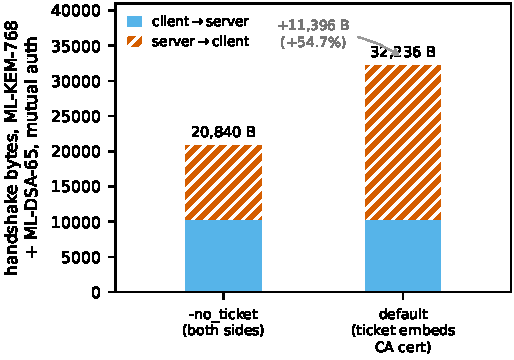
\includegraphics[width=0.62\textwidth]{m5_artefact}
\caption{The ticket artefact of Section~\ref{sec:pitfalls}, item~(5).
Both bars are the same \mlkem{}-768\,$+$\,\mldsa{}-65
mutual-authentication handshake. In the left bar the server was started
with \texttt{-no\_ticket} and the two post-handshake records are 79
bytes each. In the right bar that flag was omitted, and because
\texttt{-CAfile} is also used to build the outgoing chain, the CA
certificate is embedded in each ticket, adding 5{,}696 bytes twice.
Reporting the right-hand bar as the cost of post-quantum authentication
would have overstated it by 54.7\,\%.}
\label{fig:artefact}
\end{figure}

\begin{table}[H]
\caption{Record-level view of the artefact in
Section~\ref{sec:pitfalls}, item~(5), for
\mlkem{}-768\,$+$\,\mldsa{}-65. Server to client records are listed in
transmission order, so the last three entries of each row are the
post-handshake records. Only these three differ between the two rows.}
\label{tab:records}
\centering
\begin{tabular}{llr}
\toprule
Mode & Server$\to$client record sizes (bytes) & Total \\
\midrule
mutual auth, \texttt{-no\_ticket} & 1{,}183 6 28 107 5{,}549 3{,}339 74 79 79 24 & 10{,}468 \\
mutual auth, tickets enabled      & 1{,}183 6 28 107 5{,}549 3{,}339 74 5{,}775 5{,}775 24 & 21{,}860 \\
\bottomrule
\end{tabular}
\end{table}

Pitfall (5) is worth dwelling on for a reason beyond bookkeeping. It
pushed in the direction of our hypothesis, and a less careful
investigation would have kept it. The published literature on PQC
certificate chains reports figures in this range, and a 32\,kB handshake
is not obviously wrong. What caught it was not intuition but arithmetic:
the 5{,}759-byte records are not explicable from any field in the
handshake, and once a record cannot be attributed it has to be
investigated rather than averaged in.

\subsection{Scope: What Is Measured and What Is Not}
\label{sec:scope}

\textbf{Transport.} Every measurement here runs \tls{}~1.3 over TCP,
whereas UAV C2 links more often carry DTLS over UDP. The choice is worth
stating precisely, because it is the first question a reviewer should
ask.

The reason for TCP is not convenience: on this stack a post-quantum
DTLS handshake cannot be run at all, and the reasons are worth stating
because they are properties of the protocols rather than of our testbed.
DTLS~1.3 is specified in RFC~9147 but is not implemented in OpenSSL
3.5.7, which offers DTLS~1.0 and 1.2 only. DTLS~1.2 cannot carry the
handshake either, for two independent reasons. First, a \tls{}~1.2
cipher-suite name encodes its authentication algorithm
(\texttt{ECDHE-ECDSA-}\ldots, \texttt{ECDHE-RSA-}\ldots) and no suite
exists for \mldsa{}, so an \mldsa{} certificate cannot authenticate a
1.2-era handshake; measured, \texttt{s\_server -dtls1\_2} holding an
\mldsa{}-65 certificate answers every \texttt{ClientHello} with
\emph{no shared cipher}. Second, the 1.2 key exchange is ECDHE over an
elliptic curve and \mlkem{} is not a 1.2 group; measured,
\texttt{-groups MLKEM768 -dtls1\_2} fails the same way even with an ECDSA
certificate. Post-quantum DTLS therefore means DTLS~1.3, and on a stack
that does not implement it the choice is between measuring \tls{}~1.3
over TCP and measuring nothing.

What that costs can be bounded rather than guessed, because RFC~9147
changes framing only. Its record header is 13 bytes against 5, its
handshake header 12 against 4, and the AEAD tag is unchanged, so a
datagram of $M$ bytes carries $M-42$ bytes of handshake body. Applying
that to the measured record list --- five fragments for each 5{,}549-byte
\texttt{Certificate} at a 1{,}200-byte datagram, three for each
\texttt{CertificateVerify}, two for each hello --- gives 21{,}659 bytes
against 20{,}817, an increase of 842 bytes or 4.0\,\%
(\texttt{harness/dtls\_bound.py}; at a 1{,}000-byte datagram it is
1{,}010 bytes, 4.9\,\%). The certificate and signature records grow by
3.2\,\%, so their share of the handshake moves from 85.4 to 84.7\,\%:
the transport scales the handshake without reordering it.

Two further effects point the same way. TCP repairs a lost segment by
retransmitting that segment, whereas DTLS repairs a lost datagram by
retransmitting the whole flight it belonged to, and post-quantum flights
are necessarily large. And the numbers above are framing alone; a real
datagram path adds IP and UDP headers that the \tls{} counts here do not
include.

What survives intact is the attribution. RFC~9147 reuses the \tls{}~1.3
handshake messages unchanged, so the split between key exchange and
identity material --- the paper's main result --- is a property of the
handshake, not of the transport that carries it. The end-to-end times
are the part that would move, and they would move upward by roughly the
4\,\% above.

This bound runs along the transport dimension only, and holds loss
equal: at a given loss rate, DTLS would cost more than the numbers here,
not less. It does not cancel the opposite caveat in
Section~\ref{sec:threats}, where the emulated link is argued to be
cleaner than a real one. The two act in different directions and neither
is small; what the paper claims is the attribution and the ordering of
remedies, which survive both.

The asymmetry also fixes the sign of that error, which is the part that
matters for the ordering. The flight that carries the identity material
is about 10{,}400 bytes, nine datagrams at the 1{,}200-byte MTU used
above, whereas the pre-shared-key handshake completes in one or two
datagrams per flight. A DTLS peer that loses a datagram retransmits its
whole flight, so at equal loss probability the certificate handshake
pays several times the retransmission the pre-shared-key one does.
Section~\ref{sec:loss} measures the certificate penalty growing by
0.446\,s per injected loss on TCP; on DTLS it would grow faster while
the pre-shared-key penalty barely moved, and the gap between the two
would widen rather than close. The ordering reported here is therefore
the conservative one on the transport UAV links actually use, and the
same is true of the bursty fades that Section~\ref{sec:threats} says are
not modelled: a fade that swallows several datagrams at once costs a
large flight several whole retransmissions and a small one a single
datagram.

Measured: bytes in each direction, handshake completion time, and
per-record attribution, all on a real \tls{}~1.3 stack. Also measured:
the effect of changing the certificate signature algorithm while
holding the key exchange fixed, the effect of replacing certificates
with a pre-shared key, and how both move when the link rate varies from
2.4 to 38.4\,\kbps{} and the one-way delay from 0 to 600\,ms.

Not measured: microprocessor cycle counts, RAM footprints and energy on
the flight controller itself. What is measured is the arithmetic on the
host that runs the testbed, and the margin it implies. A
mutual-authentication \mldsa{}-65 handshake performs two signatures, two
verifications and one \mlkem{}-768 exchange; timed with
\texttt{openssl speed} on the test host these total about 1.8\,ms against
11.27\,s of transmission --- 0.02\,\%, a margin of some 6{,}000
(\texttt{harness/compute\_cost.py}). Repeat runs on the same host moved
the total by about 10\,\%, between 1.8 and 1.9\,ms, which is why the
figure is quoted to two significant digits rather than four. The heaviest
scheme measured, \mldsa{}-87, is about 2\,ms. For computation to match
transmission on this link the processor would have to be 6{,}000 times
slower than a desktop core; at a thousand times slower the arithmetic
would still be under a fifth of the handshake, and the constraint of the
link would still be the link.

That is the sense in which the premise is checkable: it is not that
computation is fast everywhere, but that it would have to be
catastrophically slow to matter, and a device that slow could not
complete a \tls{} handshake at all. Where such figures do bear on a
design decision --- the \fndsa{} signing cost in
Section~\ref{sec:compact} --- they are attributed to the literature and
used to argue against a design, not to support one.

Behaviour under bursty packet loss is also not measured, although
independent per-segment loss is: Section~\ref{sec:loss} injects
retransmission timeouts at rates up to one segment in five and finds
that the penalty is proportional to the number of segments rather than
to the handshake design. Bursty fading, in which one fade swallows
several segments at once, is not modelled and is flagged in
Section~\ref{sec:threats}.

\section{Results}
\label{sec:results}

\subsection{Where the Bytes Go}
\label{sec:attribution}

Table~\ref{tab:breakdown} and Figure~\ref{fig:breakdown} attribute every
byte of a mutual-authentication \tls{}~1.3 handshake. The attribution
uses a record-layer parser rather than a total counter, so the key
exchange is separated from the identity material exactly: the
\texttt{ClientHello} and \texttt{ServerHello} are plaintext in
\tls{}~1.3 and their lengths are read from the wire, and everything
after them is accounted by record.

\begin{table}[H]
\caption{Byte attribution of the mutual-authentication \tls{}~1.3
handshake, measured with a record-layer parser. ``Key exchange'' is the
\texttt{ClientHello} and \texttt{ServerHello} in both directions.
``Identity'' is everything else: two certificates, two
\texttt{CertificateVerify} signatures, \texttt{Finished}, and record and
message framing. All configurations use ECDSA-P256 for the classical
baseline and the stated scheme elsewhere. The identity column is a
residual --- the total minus the two hello payloads --- so it also
absorbs the 10 bytes of hello record headers and the 23-byte probe record
of Section~\ref{sec:method}; certificates and signatures proper account
for 17{,}646 of the 18{,}310. The two pre-shared-key rows carry no
certificate at all, so their residual is \texttt{Finished} and framing
only: the 316 bytes there is what a handshake costs after the identity
material is gone, not an identity overhead, and the 45.0\,\% and
10.9\,\% shares are tabulated so the column is complete rather than
because they measure identity.}
\label{tab:breakdown}
\centering
\begin{tabular}{lrrrr}
\toprule
Configuration & Key exchange & Identity & Total & Identity share \\
\midrule
X25519 $+$ ECDSA-P256        & 330  & 1{,}583  & 1{,}913  & 82.8\,\% \\
X25519 $+$ \mldsa{}-65       & 330  & 18{,}310 & 18{,}640 & 98.2\,\% \\
\mlkem{}-768 $+$ ECDSA-P256  & 2{,}530 & 1{,}585  & 4{,}115  & 38.5\,\% \\
\mlkem{}-768 $+$ \mldsa{}-65 & 2{,}530 & 18{,}310 & 20{,}840 & 87.9\,\% \\
\mlkem{}-768 PSK             & 2{,}586 & 316      & 2{,}902  & 10.9\,\% \\
X25519 PSK                   & 386  & 316      & 702      & 45.0\,\% \\
\bottomrule
\end{tabular}
\end{table}

\begin{figure}[H]
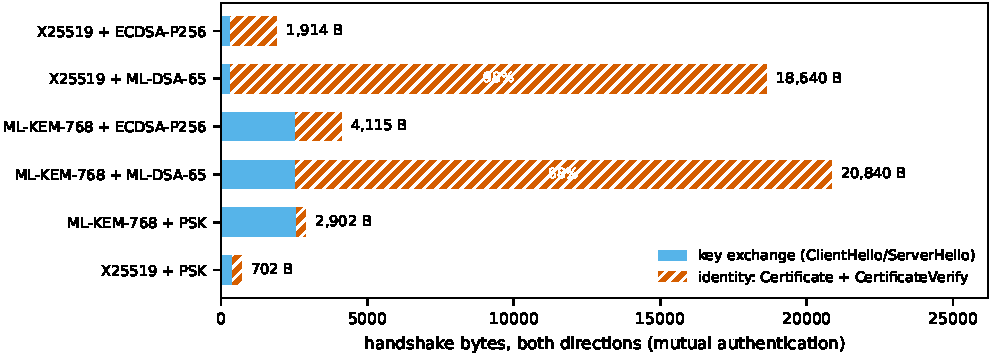
\includegraphics[width=\textwidth]{m1_breakdown}
\caption{Byte attribution of the configurations in
Table~\ref{tab:breakdown}. The key exchange is the blue segment; the
orange segment is certificate and signature material. Swapping X25519
for \mlkem{}-768 adds 2{,}202 bytes. Swapping an ECDSA-P256
certificate for an \mldsa{}-65 one adds 16{,}727 bytes. The
post-quantum key exchange is not where the bytes are, and reducing its
size is not where the leverage is.}
\label{fig:breakdown}
\end{figure}

The result is stark. Holding the certificate fixed and changing the key
exchange from X25519 to \mlkem{}-768 adds 2{,}202 bytes. Holding the
key exchange fixed and changing the certificate from ECDSA-P256 to
\mldsa{}-65 adds 16{,}727 bytes. The ratio is 7.6 to 1.

This ratio is self-consistent in a way that gives us confidence it is a
property of the protocol and not of our testbed. The identity increment
is 16{,}727, 16{,}726, 16{,}727 and 16{,}727 bytes for the four key
exchanges we tested (X25519, X25519\mlkem{}768, \mlkem{}-768,
\mlkem{}-1024) --- constant to within one byte, as it must be if the
identity material is independent of the key exchange. It also decomposes
as theory requires: an \mldsa{}-65 certificate is 5{,}514 bytes of DER
against 389 for the ECDSA one, and a \texttt{CertificateVerify}
signature is 3{,}309 bytes against 71. Doubling both for mutual
authentication gives $2\times(5{,}514+3{,}309) - 2\times(389+71) =
16{,}726$ bytes, which is the measured column increment of
Table~\ref{tab:matrix} to the byte.
Section~\ref{sec:arithmetic} carries the same reconstruction down to
individual messages.

\begin{table}[H]
\caption{Full measured matrix: handshake bytes and completion time (s)
for every combination of four key exchanges and four certificate
signature algorithms, mutual authentication, 9.6\,\kbps{} per direction
and 250\,ms one-way. Cells are single runs; the repeatability of
Section~\ref{sec:repeat} puts a $1\sigma$ interval of about $\pm0.02$\,s
on each, which is smaller than the last digit shown. The row and column
increments are additive to within $\pm 2$ bytes, which is the property
Section~\ref{sec:attribution} relies on.}
\label{tab:matrix}
\centering
\begin{tabular}{lrrrr}
\toprule
Key exchange & ECDSA-P256 & \mldsa{}-44 & \mldsa{}-65 & \mldsa{}-87 \\
\midrule
X25519          & 1{,}915 / 1.99  & 13{,}804 / 7.19 & 18{,}640 / 9.45  & 25{,}192 / 12.44 \\
X25519\mlkem{}768 & 4{,}177 / 3.86 & 16{,}068 / 9.07 & 20{,}904 / 11.33 & 27{,}456 / 14.31 \\
\mlkem{}-768    & 4{,}114 / 3.81  & 16{,}004 / 9.02 & 20{,}840 / 11.27 & 27{,}392 / 14.27 \\
\mlkem{}-1024   & 4{,}979 / 4.54  & 16{,}868 / 9.97 & 21{,}704 / 12.00 & 28{,}256 / 14.99 \\
\midrule
\multicolumn{5}{l}{\emph{Column increment over ECDSA-P256, by row}} \\
X25519          & -- & 11{,}889 & 16{,}725 & 23{,}277 \\
\mlkem{}-768    & -- & 11{,}890 & 16{,}726 & 23{,}278 \\
\midrule
\multicolumn{5}{l}{\emph{Row increment over X25519, by column}} \\
\mldsa{}-65      & 2{,}199 & 2{,}200 & 2{,}200 & 2{,}200 \\
\mlkem{}-1024   & 3{,}064 & 3{,}064 & 3{,}064 & 3{,}064 \\
\bottomrule
\end{tabular}
\end{table}

Table~\ref{tab:matrix} is the evidence for treating the two halves of
the handshake as independent. Reading down a column gives the cost of
the key exchange and is constant to within one byte regardless of which
certificate is used; reading across a row gives the cost of the
certificate and is constant to within two bytes regardless of which key
exchange is used. The two byte costs add. This is what makes it
legitimate to say that the certificate costs 16{,}726 bytes rather than
that the configuration costs 20{,}840: the decomposition is not a
modelling assumption, it is a measured invariance.

The residual $\pm 2$ bytes is DER encoding noise, and it is classical
only. \mldsa{} signatures are fixed-length byte strings, so a
post-quantum total is exactly reproducible: 20{,}840 in every run we
made. The classical baseline is not, because an ECDSA signature is
variable-length DER --- the integers $r$ and $s$ gain a leading zero
byte whenever the value behind them is small --- so the certificate and
each \texttt{CertificateVerify} move by a byte or two between runs.
The classical baseline measures 1{,}912, 1{,}913, 1{,}915 and 1{,}916
bytes in the batches behind Tables~\ref{tab:loss},
\ref{tab:breakdown}, \ref{tab:matrix} and \ref{tab:repeat}
respectively. Each table reports the values from the batch that
produced it, and \emph{ratios are compared only within one batch}: the
certificate penalty is 5.66$\times$ in the sweep of
Table~\ref{tab:matrix} and 5.67$\times$ in the repeats of
Table~\ref{tab:repeat}, a spread of 0.2\,\%, and no conclusion
depends on which baseline is used.

\subsection{Where the 20{,}840 Bytes Come From}
\label{sec:arithmetic}

The attribution above is only credible if the individual messages can be
reconstructed from the standards, so Table~\ref{tab:messages} does that.
Two observations follow. First, the two directions are almost symmetric
--- 10{,}372 and 10{,}468 bytes --- which is what mutual authentication
implies, and which is why the cost of the identity material is paid
twice. Second, the certificate dominates every other message in the
handshake: at 5{,}549 bytes it is 4.7 times the next largest, and there
are two of them.

\begin{table}[H]
\caption{Per-message reconstruction of the measured handshake
(\mlkem{}-768\,$+$\,\mldsa{}-65, mutual authentication). Every figure in
the `bytes' column is read off the wire by the record-layer parser;
every figure in the `contents' column is from FIPS~203/204 plus X.509
and \tls{} framing, so the two can be checked against each other. The
`framing' rows hold the records that carry no identity material:
\texttt{ChangeCipherSpec}, the one-byte application probe of
Section~\ref{sec:method}, and the post-handshake records. Byte counts in
this table include the 5-byte \tls{} record header; the key-exchange
totals quoted in the text are payload-only and are therefore 10 bytes
smaller for the two hello messages, which is the 2{,}530 of
Table~\ref{tab:breakdown}. Every row decomposes exactly: the 5{,}549-byte
\texttt{Certificate} is 35 bytes of \tls{} framing --- 5 record header,
16 AEAD tag, 4 handshake header, 1 content type, 1 context length,
3 list length, 3 certificate length and 2 extensions length --- plus the
5{,}514-byte DER, which in turn is 1{,}952 of public key, 3{,}309 of
signature and 253 of X.509 frame.} 
\label{tab:messages}
\centering
\small
\begin{tabular}{llrl}
\toprule
Direction & Message & Bytes & Contents \\
\midrule
\multirow{5}{*}{client$\to$server}
 & \texttt{ClientHello}      & 1{,}357 & of which key share 1{,}192 \\
 & \texttt{Certificate}      & 5{,}549 & DER 5{,}514 $+$ 35 framing \\
 & \texttt{CertificateVerify}& 3{,}339 & signature 3{,}309 $+$ 30 framing \\
 & \texttt{Finished}         & 74      & \\
 & framing                 & 53      & CCS 6, probe 23, close 24 \\
\midrule
\multirow{6}{*}{server$\to$client}
 & \texttt{ServerHello}      & 1{,}183 & of which key share 1{,}096 \\
 & \texttt{EncryptedExtensions} & 28   & \\
 & \texttt{CertificateRequest} & 107 & \\
 & \texttt{Certificate}      & 5{,}549 & as above \\
 & \texttt{CertificateVerify}& 3{,}339 & as above \\
 & \texttt{Finished} and framing & 262 & Finished 74, CCS 6, tickets 158, close 24 \\
\midrule
\multicolumn{2}{l}{Total, both directions} & 20{,}840 & \\
\bottomrule
\end{tabular}
\end{table}

Taking the two hello messages as the key-exchange term, consistently
with Table~\ref{tab:breakdown}, they total 2{,}530 bytes or 12.1\,\%
of the handshake; of those, 2{,}288 carry the actual key material
(1{,}184 bytes of \mlkem{} public key and 1{,}088 of ciphertext, plus
extension headers) and the rest is \tls{} machinery. The identity
material is 18{,}310 bytes. The mechanism is therefore visible per
message as well as in aggregate: it is not that \mlkem{} is large, it
is that there are two certificates and two signatures, and each of the
four is larger than the entire key exchange.

The two ratios quoted in the introduction differ for a reason worth
naming. The 7.8 uses the standard object sizes alone, 17{,}646 against
2{,}272; the 7.2 uses what the wire carries, 18{,}310 against 2{,}530.
Framing raises both terms but the smaller one faster --- 2{,}272 to
2{,}530 is 11.4\,\%, 17{,}646 to 18{,}310 is 3.8\,\% --- so the ratio
a packet shows is the lower of the two. Neither is an error; a paper
that quoted only the higher one would be quoting a number no link can
produce.

\textbf{Mutual authentication turns out to be almost free, which is a
result rather than an oversight.} Every number above authenticates both
ends. A reader may reasonably ask what authenticating one direction
would save, since an uplink that dials a known server is a common shape
and \mav{} signing is sometimes offered as the aircraft-side check. We
measured it (\texttt{results/oneway.csv}): omitting the client
certificate removes 8{,}995 of the 20{,}840 bytes, 43\,\%, and 0.10\,s
of the 11.28\,s. The bytes fall by nearly half and the time barely
moves, because completion time is set by the longest flight in either
direction rather than by the total. The server's flight is 10{,}468
bytes with a client certificate on the wire and 10{,}361 without --- the
certificate the server sends does not shrink --- so the client's
certificate rides in parallel with a wait that was going to happen
anyway. Mutual authentication starts to cost something only when the
client's flight would exceed the server's, and at these sizes it does
not.

Two consequences follow. The first is that the mutual-authentication
numbers throughout this paper are the conservative ones, and an operator
cannot buy airtime back by authenticating one direction only. The second
is a change in the split: with one direction authenticated, the identity
share falls from 87.9 to 78.6\,\%, because the 2{,}530 bytes of key
exchange are not halved along with the certificates. That is a change in
the denominator, not in the remedy --- identity still dominates, and the
three remedies retain their order.

\subsection{The Certificate Parameter Sweep}
\label{sec:sweep}

\mldsa{} has three parameter sets, and because they differ only in
security level they provide a controlled probe of how bytes convert
into time. Table~\ref{tab:sweep} reports all four certificate
algorithms at a fixed key exchange.

\begin{table}[H]
\caption{Handshake size and completion time for mutual authentication,
\mlkem{}-768 key exchange, varying certificate signature algorithm
(9.6\,\kbps{} per direction, 250\,ms one-way). Times are single runs;
the fifth column is the sample standard deviation over five repeats of
the same cell on the same link (\texttt{results/sweep\_repeat.csv}),
whose mean lies within 0.03\,s of the single-run time in the same row,
and the final column is the byte difference between adjacent rows
divided by the time difference. The classical row is the only one whose byte count moves
between batches, for the reason Section~\ref{sec:attribution} gives.}
\label{tab:sweep}
\centering
\small
\begin{tabular}{lrrrrr}
\toprule
Certificate & Bytes & 9.6\,\kbps{} (s) & 64\,\kbps{} (s) & sd, 5 runs & Marginal (B/s) \\
\midrule
ECDSA-P256   & 4{,}114  & 3.81  & 0.58 & 0.024 & -- \\
\mldsa{}-44  & 16{,}004 & 9.02  & 1.74 & 0.018 & 2{,}282 \\
\mldsa{}-65  & 20{,}840 & 11.27 & 2.08 & 0.012 & 2{,}150 \\
\mldsa{}-87  & 27{,}392 & 14.27 & 2.45 & 0.013 & 2{,}183 \\
\bottomrule
\end{tabular}
\end{table}

\begin{figure}[H]
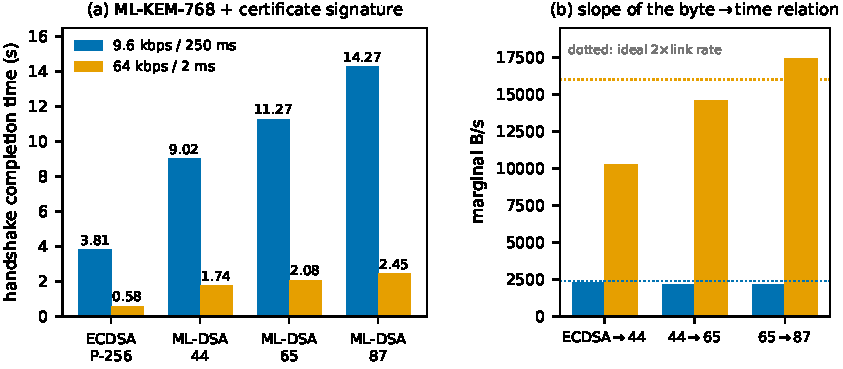
\includegraphics[width=\textwidth]{m2_sweep}
\caption{(a) Completion time for the sweep of Table~\ref{tab:sweep} at
two link rates. (b) The slope of the same sweep, computed as the byte
difference between adjacent certificate algorithms divided by the time
difference. At 9.6\,\kbps{} the slope is stable at 2{,}150--2{,}282\,B/s,
which is 90--95\,\% of the ideal 2{,}400\,B/s obtained if both directions
serialise in parallel at the link rate. This stability is what licenses
the extrapolation in Figure~\ref{fig:ladder}; at 64\,\kbps{} the same
slope scatters by a factor of 1.7, so we do not extrapolate from that
rate.}
\label{fig:sweep}
\end{figure}

Figure~\ref{fig:sweep}(b) is the reason this sweep is worth reporting
rather than merely listing. The marginal throughput at 9.6\,\kbps{} is
2{,}282, 2{,}150 and 2{,}183\,B/s for the three steps, a spread of
1.5\,\%. The ideal value, if both directions serialise in parallel at
the link rate, is $2 \times 1{,}200 = 2{,}400$\,B/s; the measured values
are 90--95\,\% of it, the shortfall being \tls{} and TCP framing. At
64\,\kbps{} the same computation gives 10{,}236, 14{,}572 and
17{,}425\,B/s, a spread of 70\,\%, because at that rate the fixed
protocol overheads are comparable to the transfer itself.

The practical consequence is a conversion rule with a stated domain of
validity. On a 9.6\,\kbps{} link with 250\,ms propagation, adding a
byte to a handshake costs $1/2{,}200 \approx 0.45$\,ms. That rule can
be used to predict configurations we cannot measure directly, which is
what Section~\ref{sec:compact} does; it should not be used at rates
where the fixed overheads dominate.

\subsection{How the Penalty Moves with Link Rate}
\label{sec:rate}

Every measurement so far is at 9.6\,\kbps{} per direction. A byte-count
penalty should shrink as a link speeds up, so a reader is entitled to
ask whether the 5.66$\times$ of Table~\ref{tab:psk} is an artefact of
having chosen a slow link. We tested that by varying one thing: rate
from 2.4 to 38.4\,\kbps{} in five steps, with the 250\,ms one-way delay
held fixed, so that every point describes the same geostationary link
at a different transponder bandwidth. That is how satellite C2 capacity
is actually bought, so the sweep corresponds to a procurement decision
an operator will face. Two runs per cell.

\begin{table}[H]
\caption{Completion time against link rate at a fixed 250\,ms one-way
delay. Cells are mean handshake bytes / mean completion time in
seconds over two runs. Two is fewer than elsewhere in the paper, and the
justification is the measured spread rather than convenience: across the
fifteen cells the largest within-cell difference is 1.9\,\% and the
median 0.3\,\%, both far below the 2.8$\times$ range the table exists to
show. ``PQC'' is \mlkem{}-768$+$\mldsa{}-65,
``pre-shared'' is \mlkem{}-768 with an external PSK. Ratios are formed
within each row, so they are unaffected by the inter-run byte variation
of Section~\ref{sec:attribution}.}
\label{tab:rate}
\centering
\small
\begin{tabular}{lrrrrr}
\toprule
Rate & Classical & PQC & Pre-shared & PQC / & PSK / \\
(kbps) & & & key & classical & classical \\
\midrule
2.4  & 1{,}913 / 4.68  & 20{,}658 / 40.43 & 2{,}902 / 10.09 & 8.64$\times$ & 2.16$\times$ \\
4.8  & 1{,}915 / 2.88  & 20{,}840 / 20.99 & 2{,}902 / 5.56  & 7.29$\times$ & 1.93$\times$ \\
9.6  & 1{,}913 / 1.98  & 20{,}840 / 11.27 & 2{,}902 / 3.37  & 5.70$\times$ & 1.70$\times$ \\
19.2 & 1{,}912 / 1.56  & 20{,}840 / 6.41  & 2{,}902 / 2.18  & 4.11$\times$ & 1.40$\times$ \\
38.4 & 1{,}913 / 1.30  & 20{,}840 / 3.98  & 2{,}902 / 1.61  & 3.07$\times$ & 1.24$\times$ \\
\bottomrule
\end{tabular}
\end{table}

\begin{figure}[H]
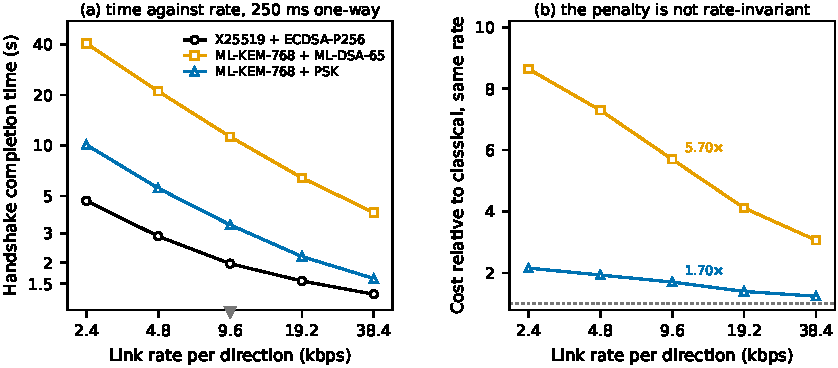
\includegraphics[width=\textwidth]{m7_rate}
\caption{Rate sweep at a fixed 250\,ms one-way delay. (a) Completion
time against rate on logarithmic axes; the small triangle below the
axis marks the 9.6\,\kbps{} DO-362 operating point used everywhere else
in this paper. A handshake bound purely by serialisation would follow a
line of slope $-1$; the measured lines are steeper at the low end and
flatten at the high end, which is a fixed cost being overtaken by a
rate-proportional one. (b) The same data expressed as a cost relative
to the classical baseline at the same rate. The certificate penalty is
not rate-invariant: it falls from 8.64$\times$ to 3.07$\times$ across
the sweep. The pre-shared-key penalty falls more gently, from
2.16$\times$ to 1.24$\times$, because it has removed most of the bytes
that scale with rate. The annotated 9.6\,\kbps{} values (5.70$\times$ and
1.70$\times$) belong to this sweep's own baseline of 1.98\,s and are
therefore 0.7\,\% and 1.8\,\% above the 5.66$\times$ and 1.67$\times$ of
Table~\ref{tab:psk}, which comes from a different batch; see the batch
rule in Section~\ref{sec:attribution}.}
\label{fig:rate}
\end{figure}

Figure~\ref{fig:rate} plots the sweep, both as absolute completion time
and as the same data expressed relative to the classical baseline at each
rate. The figure is its own batch, so its ratios sit 0.7\,\% and
1.8\,\% above the 5.66$\times$ and 1.67$\times$ of
Table~\ref{tab:psk}; the batches differ only in the ECDSA baseline, for
the reason Section~\ref{sec:attribution} gives.

\textbf{The penalty is not a constant, and the earlier draft of this
paper said it was.} It falls monotonically from 8.64$\times$ at
2.4\,\kbps{} to 3.07$\times$ at 38.4\,\kbps{}. The 5.66$\times$ that
organises most of the discussion above is therefore the value \emph{at
one operating point}, not a property of the handshake. Reporting it
without the sweep would have overstated the migration cost at high rate
and understated it at low rate, and the understatement matters more,
because it is the narrow links that need the migration most.

\textbf{Why the ratio moves while the byte difference does not.} The
byte gap is 18{,}928 bytes in four of the five rows and 18{,}745 in the
2.4\,\kbps{} row. Two separate artefacts push that row 183 bytes lower:
its pre-shared-key-free handshake counts 182 bytes fewer, and its
classical baseline counts one byte more. Both are the window-boundary
effect described at the end of this subsection, and neither changes a
ratio in the third significant figure. What changes is how much of the
completion time is serialisation. At 38.4\,\kbps{} the
classical handshake takes 1.30\,s, of which serialising its larger
direction (1{,}048 bytes) accounts for 0.22\,s; at 2.4\,\kbps{} it
takes 4.68\,s against 3.49\,s. The ratio of measured to
serialisation-only time therefore rises from 1.34 to 6.0 as the link
speeds up, and the fixed cost --- two propagation legs plus the
handshake round trips --- is diluted by a denominator that has stopped
growing. The absolute gap tracks serialisation instead: it widens
thirteen-fold, from 2.68\,s at 38.4\,\kbps{} to 35.75\,s at
2.4\,\kbps{}, while the bytes responsible for it do not move at all.

\textbf{The pre-shared-key option is far less rate-sensitive.} Its
penalty falls only from 2.16$\times$ to 1.24$\times$, because 87.9\,\%
of the certificate handshake's bytes are gone and with them most of the
term that scales with rate. This strengthens rather than weakens the
design rule of Section~\ref{sec:psk}: the architecture choice is worth
2.5$\times$ in time at 38.4\,\kbps{} and 4.0$\times$ at 2.4\,\kbps{},
against the 1.25$\times$ that the largest signature-algorithm change
available (\mldsa{}-65 down to \mldsa{}-44) delivers at 9.6\,\kbps{}
--- and the certificate rows of Table~\ref{tab:rate} show the penalty
growing, not shrinking, as the link narrows, so the gap between the two
kinds of remedy only widens as the link gets harder.

One number needs a caveat. The 2.4\,\kbps{} row counts 20{,}658 bytes
rather than 20{,}840, 0.9\,\% fewer. The record decomposition at that
rate is identical to the one at 9.6\,\kbps{} (same record lengths, same
order), so the difference is a counting artefact at the measurement
window boundary rather than a differently framed handshake. At
2.4\,\kbps{} those 182 bytes are worth 0.61\,s, which is 1.5\,\% of
the 40.43\,s in that row; the ratio we report for the row would move in
the third significant figure and we quote it to two decimals
accordingly.

\subsection{How the Penalty Moves with Link Delay}
\label{sec:delay}

The sweep above varies bandwidth at a fixed 250\,ms delay, which leaves
a second objection open: apart from that sweep, every number in this
paper describes one geostationary link. An operator flying a low Earth
orbit constellation will want to know whether the 5.66$\times$ survives
a 20--60\,ms path, and whether ``bandwidth is the binding constraint''
survives a link whose latency is small.

One caveat belongs before the numbers rather than in the caption.
The emulator charges its configured delay once per forwarded chunk rather
than once per direction switch, so the \emph{absolute} slope of time
against delay is a property of the emulator, not of the link, and cannot
be compared with a real satellite budget. What is transport-independent
is the ratio between two configurations measured on the same emulator,
and that is all this section reads from the table.

We varied the one-way delay and held everything else fixed: 9.6\,\kbps{}
per direction, three configurations, four delays, three runs per cell,
one batch. Zero delay isolates serialisation; 40\,ms is a low Earth
orbit pass; 250\,ms is geostationary; 600\,ms is geostationary with a
second hop through a ground station, which is the topology an operator
with a remote control centre actually builds. Table~\ref{tab:delay}
gives the result.

\begin{table}[H]
\caption{Completion time against one-way propagation delay at a fixed
9.6\,\kbps{} per direction. Cells are means over three runs; the largest
standard deviation in the table is 0.014\,s. ``PQC'' is
\mlkem{}-768$+$\mldsa{}-65, ``pre-shared'' is \mlkem{}-768 with an
external PSK. Ratios are formed within each row. This is a third batch,
so its 250\,ms row reads 5.76$\times$ where Table~\ref{tab:psk} reads
5.66$\times$ and Table~\ref{tab:rate} 5.70$\times$; the byte counts are
identical and the difference is the classical baseline of
Section~\ref{sec:attribution}. The slope these rows imply is a property
of how the emulator charges delay, not of the handshake; only the ratio
between the two slopes is read as a link property
(Section~\ref{sec:delay}).}
\label{tab:delay}
\centering
\small
\begin{tabular}{llrrrrr}
\toprule
Delay & Link & Classical & PQC & Pre-shared & PQC / & PSK / \\
(ms) & & (s) & (s) & key (s) & classical & classical \\
\midrule
0   & control, no propagation & 1.47  & 10.27 & 2.44 & 7.00$\times$ & 1.66$\times$ \\
40  & low Earth orbit         & 1.55  & 10.43 & 2.62 & 6.71$\times$ & 1.69$\times$ \\
250 & geostationary           & 1.96  & 11.27 & 3.31 & 5.76$\times$ & 1.69$\times$ \\
600 & geostationary, two hops & 2.68  & 12.67 & 4.00 & 4.72$\times$ & 1.49$\times$ \\
\bottomrule
\end{tabular}
\end{table}

\textbf{Two things move in opposite directions, and until now this
paper has been quoting the one that flatters the technology.} Completion time is linear in delay to
within 14\,ms across the four rows, with a slope of 4.00\,s per second
of one-way delay for the certificate handshake, 2.03 for the classical
baseline and 2.59 for the pre-shared-key one. The certificate
configuration therefore places twice as much of its work behind a
propagation delay as the classical one, and the absolute gap between
them \emph{widens}, from 8.80\,s at zero delay to 9.99\,s at 600\,ms.
Latency does not rescue the certificate handshake; it adds to it.

The ratio, however, falls from 7.00$\times$ to 4.72$\times$, because the
classical baseline nearly doubles over the same interval (1.83$\times$)
while the post-quantum total grows by 1.23$\times$. The byte gap is
constant at every delay; what changes is the common additive term that
latency contributes, which inflates a smaller denominator
proportionally more. This is the same mechanism as in the rate sweep,
with latency in place of rate, and it produces the same kind of
movement in the ratio and the same stability in the bytes.

\textbf{The consequence is that the headline figure is conservative.}
The ratio falls monotonically with delay, so for any link with no more
than 250\,ms of one-way propagation --- low Earth orbit, medium Earth
orbit, or a single geostationary hop --- the certificate penalty is at
least the 5.66$\times$ of Table~\ref{tab:psk}: 6.71$\times$ at 40\,ms
and 7.00$\times$ at zero delay. Only the two-hop path buys the ratio
down to 4.72$\times$, and it pays for that with an absolute penalty
0.7\,s larger than the geostationary one. A reader who deploys over low
Earth orbit should expect the ratio of Section~\ref{sec:attribution},
not a smaller one, and the absolute penalty of 8.9\,s there is within
0.5\,s of the geostationary figure. The claim that narrow links are where the
certificate penalty bites is thus reinforced rather than qualified: the
links with the least latency are the ones where it is largest relative
to the baseline they replace.

Three caveats bound this table. The slope counts chunk-level delay
payments, because the proxy holds each forwarded chunk for one one-way
delay (Section~\ref{sec:link}); the absolute value 4.00 is therefore a
property of the emulator, and only the ratio of slopes --- twice the
classical figure --- is interpretable as a property of the handshake.
Zero delay is a control and not a link: no radio path has none, and the
row exists to separate serialisation from propagation. And the table
is a batch of its own, as the caption states.

\subsection{Pre-Provisioned Trust}
\label{sec:psk}

The sweep suggests that shrinking the certificate is expensive per byte
saved. The alternative is to not send a certificate at all. A
\tls{}~1.3 external pre-shared key authenticates both endpoints and
establishes fresh key material without any certificate, any
\texttt{CertificateVerify} and any trust anchor on the link.

Table~\ref{tab:psk} reports the comparison. The pre-shared-key
handshake carries 2{,}902 bytes and completes in 3.32\,s, against
20{,}840 bytes and 11.29\,s for certificate authentication: 7.2$\times$
less traffic and 3.4$\times$ less time. It retains \mlkem{}-768 for key
exchange, because \tls{}~1.3 pre-shared-key mode uses
\texttt{psk\_dhe\_ke} by default and therefore keeps the post-quantum
contribution to forward secrecy. The records confirm the mode: the
client's \texttt{ClientHello} grows by exactly 50 bytes, which is the
\texttt{pre\_shared\_key} extension, while the server still returns a
1{,}088-byte \mlkem{} ciphertext. The 17{,}938 bytes saved are therefore
identity material, not key exchange. What it gives up is identity: the
peers are authenticated by possession of the pre-shared key, not by a
certificate chain.

Two things follow that the byte count does not show, and both cut against
reading the 7.2$\times$ as a free saving. The first is that the risk is
concentrated rather than created: a pre-shared key authenticates every
session that holds it, so its compromise is the compromise of the whole
fleet at once, whereas one aircraft's signing key opens one aircraft.
The radius follows from the topology rather than from the crypto: in the
twenty-aircraft, three-station fleet of Section~\ref{sec:keymgmt} a
captured aircraft key opens three links for the weeks it takes to re-key
them, and a group key used instead of pairwise keys opens all sixty
endpoints for the same window. The
second is that the certificate has a revocation channel and the
pre-shared key does not. A certificate can be withdrawn and the peer can
be told; a key can only be replaced, and replacing it means reaching every
aircraft. The bytes of that channel are not in any table here --- a CRL or
an OCSP response on the same 9.6\,\kbps{} link is itself hundreds to
thousands of bytes --- so the comparison is of airtime per handshake, not
of lifecycle cost, and the two are not commensurable on the evidence
collected.

\begin{table}[H]
\caption{Certificate authentication versus pre-provisioned trust, mutual
authentication, 9.6\,\kbps{} per direction, 250\,ms one-way. The
classical baseline is included for scale. The pre-shared-key
configuration keeps \mlkem{}-768 for key exchange and drops only the
identity material. Its 2{,}902 bytes comprise 330 bytes of hello common
to every configuration, 56 bytes of pre-shared-key extension and
2{,}200 bytes of \mlkem{}-768 exchange, so the 1{,}088-byte ciphertext
is still on the wire; that is what preserves forward secrecy, and it is
why the saving is 3.4$\times$ rather than the 30$\times$ that also
dropping the post-quantum exchange would give. The classical baseline
is 1.99\,s from the same batch, so the 5.66$\times$ here is formed
against that; Figure~\ref{fig:rate} quotes 5.70$\times$ from the rate
sweep's own 1.98\,s baseline.}
\label{tab:psk}
\centering
\begin{tabular}{lrrr}
\toprule
Configuration & Handshake bytes & Time (s) & Relative to classical \\
\midrule
X25519 $+$ ECDSA-P256 (classical) & 1{,}915 & 1.99 & 1.00$\times$ \\
\mlkem{}-768 $+$ \mldsa{}-65       & 20{,}840 & 11.29 & 5.66$\times$ \\
\mlkem{}-768 $+$ pre-shared key    & 2{,}902 & 3.32 & 1.67$\times$ \\
\bottomrule
\end{tabular}
\end{table}

\begin{figure}[H]
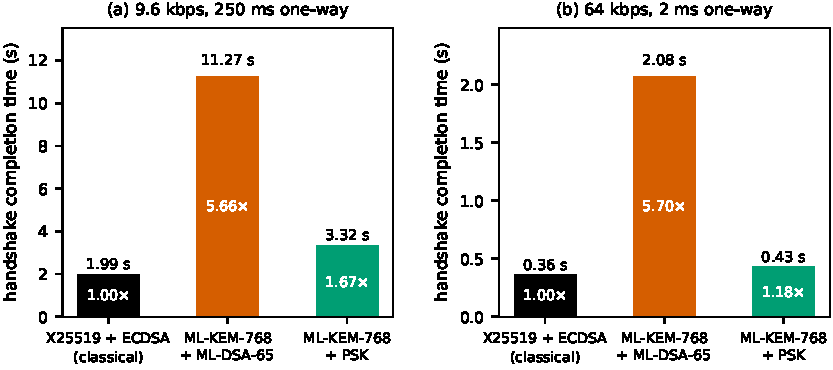
\includegraphics[width=\textwidth]{m3_architecture}
\caption{The same three configurations on two different links: a
250\,ms, 9.6\,\kbps{} beyond-line-of-sight link and a 2\,ms,
64\,\kbps{} line-of-sight one. The certificate handshake costs
5.66$\times$ the classical baseline on the first and 5.70$\times$ on
the second, the pre-shared-key handshake 1.67$\times$ and
1.18$\times$. The near-identity of the certificate penalty across two
very different links is a coincidence of two opposing effects, a faster
link shrinking the serialisation term but also the fixed term;
Section~\ref{sec:rate} isolates them by holding the delay fixed.}
\label{fig:arch}
\end{figure}

Figure~\ref{fig:arch} repeats the comparison on the line-of-sight
link of Section~\ref{sec:background}: 64\,\kbps{} and 2\,ms. The
certificate penalty is almost unchanged, 5.70$\times$ against
5.66$\times$, but that agreement should not be read as the penalty
being rate-invariant, because the two links differ in delay as well as
in rate and the two effects happen to cancel.
Section~\ref{sec:rate} separates them by holding the delay fixed, and
finds the penalty ranging from 3.07$\times$ to 8.64$\times$. What does
transfer between links is the ordering: the pre-shared-key penalty
falls from 1.67$\times$ to 1.18$\times$, because on the faster link
the handshake is short enough that fixed protocol overheads rather than
payload dominate.

\subsection{Link Loss: What It Changes and What It Does Not}
\label{sec:loss}

Every measurement above is on a clean link, which is the least
favourable case for our own argument: loss forces retransmission, a
certificate is 5{,}500 bytes and therefore more segments that can be
lost, so the natural prediction is that loss amplifies the certificate
penalty. We tested that prediction and it is only half right.

A TCP proxy cannot drop a byte without corrupting the stream, and DTLS
--- which could drop datagrams honestly --- is unavailable in this
OpenSSL build, which offers only DTLS 1.0 and 1.2 and in any case
failed to complete even a classical handshake in our environment. We
therefore inject loss as a retransmission timeout: with probability $p$
a chunk is held for one RTO of 1.2\,s instead of being delivered, which
reproduces the time-axis effect of a lost segment while leaving the byte
stream intact. Loss is counted per 1{,}460-byte segment rather than per
proxy chunk, because counting per chunk makes a 20{,}840-byte handshake
suffer the same loss count as a 1{,}912-byte one --- an earlier version
of this experiment did exactly that and concluded, wrongly, that loss
does not interact with handshake size.

\begin{table}[H]
\caption{Effect of link loss at 9.6\,\kbps{} and 250\,ms, eight runs per
cell, mutual authentication. ``Losses'' is the mean number of injected
retransmission timeouts actually suffered, measured, not assumed; it
scales with the segment count rather than with $p$ alone. Times are in
seconds.}
\label{tab:loss}
\centering
\begin{tabular}{lrrrrrr}
\toprule
Configuration & Bytes & Losses & Clean & $p{=}0.20$ & $\Delta T$ & $\Delta T$ \\[-2pt]
 & & & mean & mean & (s) & (\%) \\
\midrule
X25519 $+$ ECDSA-P256        & 1{,}912  & 1.0 & 1.96  & 2.41  & $+$0.45 & $+$22.8 \\
\mlkem{}-768 pre-shared key  & 2{,}902  & 1.0 & 3.31  & 3.75  & $+$0.44 & $+$13.4 \\
\mlkem{}-768 $+$ \mldsa{}-44 & 16{,}004 & 2.6 & 9.01  & 10.35 & $+$1.34 & $+$14.9 \\
\mlkem{}-768 $+$ \mldsa{}-65 & 20{,}840 & 3.4 & 11.28 & 12.61 & $+$1.34 & $+$11.9 \\
\bottomrule
\end{tabular}
\end{table}

\begin{figure}[H]
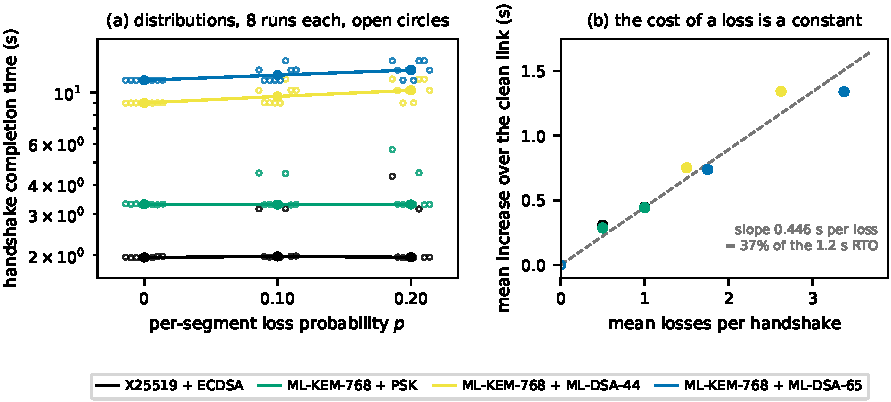
\includegraphics[width=\textwidth]{m6_loss}
\caption{Link loss. (a) Completion time against per-segment loss
probability; each open circle is one of eight runs, the filled circles
and lines are the medians. The medians barely move while the spread
grows, which is why a single run per cell would be misleading. (b) The
mean increase over the clean link, for all twelve
configuration-by-loss-rate points, against the number of injected
retransmission timeouts actually suffered. The points fall on a line
through the origin of slope $0.446$\,s per loss --- 37\,\% of the 1.2\,s
timeout, the rest being absorbed by the reverse direction. Since losses
in turn scale with segment count, this is the mechanism by which a
larger handshake pays more: not a larger per-loss cost, but more
losses.}
\label{fig:loss}
\end{figure}

Three things follow from Table~\ref{tab:loss} and
Figure~\ref{fig:loss}.

\textbf{The cost of a loss is a constant, and it is not the whole RTO.}
Across all twelve configuration-by-loss-rate points, the mean increase
in completion time is $0.446$\,s per injected loss, against an injected
1.2\,s: 37\,\% of the timeout reaches the critical path, because a loss
that lands while the peer is still transmitting in the other direction
is partly absorbed. Figure~\ref{fig:loss}(b) plots every point against
the losses actually suffered and they collapse onto that single line
through the origin, to within 0.2\,s. The penalty is therefore a
property of the link, not of the handshake.

\textbf{What varies between handshake designs is how many losses they
incur.} A 1{,}912-byte handshake spans one to two segments and suffers
one loss at $p=0.20$; a 20{,}840-byte handshake spans sixteen --- eight
in each direction, because the proxy charges every forwarded chunk at
least one segment and rounds a 4{,}096-byte read up to three --- and
suffers 3.4, against the 3.2 that sixteen segments at $p=0.20$ predict.
Multiplying by 0.446\,s gives the observed $+$0.45 and
$+$1.34\,s. Loss does amplify the certificate penalty, but only through
the segment count, and the amplification is modest: 1.34\,s against the
9.3\,s that the identity material costs in the first place.

\textbf{The ranking does not change, and the gap between the two
architectures is stable.} Comparing like with like --- every
configuration at the same loss rate --- \mlkem{}-768$+$\mldsa{}-65 costs
5.23$\times$ the classical baseline at $p=0.20$, against 5.75$\times$ at
$p=0$ in the same sweep, and the pre-shared-key case costs 1.56$\times$
against 1.69$\times$ at $p=0$. The $p=0$ figures come from the loss
sweep's own baseline and therefore differ slightly from the
5.66$\times$ and 1.67$\times$ of Table~\ref{tab:psk}; see the
batch rule in Section~\ref{sec:attribution}. Both ratios fall rather than rise, because the classical
handshake is small enough that a fixed 0.45\,s penalty is a larger
fraction of it; a first version of this comparison divided the lossy
post-quantum figure by the clean classical one and produced 6.43$\times$,
which is an artefact of mixing conditions. What carries the argument is
the ratio between the two post-quantum options, and that is essentially
unchanged: 3.41$\times$ on a clean link, 3.36$\times$ at $p=0.20$. Loss
widens the absolute gap from 9.31 to 10.20\,s but buys back none of what
pre-provisioning saves. On a link losing one segment in five,
pre-shared keys remain 3.4$\times$ cheaper in time and 7.2$\times$ in
bytes.

One observation cuts the other way and is worth stating because it
constrains how these numbers should be quoted. Loss does not shift the
median much --- the pre-shared-key median is unchanged at 3.31\,s
between $p=0$ and $p=0.20$, and the \mldsa{}-65 median moves from 11.27
to 12.47\,s --- but it moves the mean, and it moves the maximum more.
The classical baseline at $p=0.20$ has a median of 1.96\,s and a worst
observed run of 4.36\,s, a spread of 2.2$\times$ from the same
configuration. A retransmission does not merely add latency; it
triggers congestion control, and the resulting stall can exceed one
RTO. Quoting a mean, or a single run, conceals this. It is the reason
Section~\ref{sec:repeat} reports distributions rather than point
estimates, and the reason a link budget for an atomic transaction should
be set from a high quantile.

The model has two limitations, and they can be netted off rather than
merely confessed. The per-segment loss draw is binomial and independent,
so it cannot represent the bursty fading that dominates a real
narrowband radio link; and charging one RTO per lost segment is an upper
bound, since a real TCP retransmits several losses within one timeout
using SACK. Take a Gilbert--Elliott channel whose bad state loses every
segment, with stationary loss rate $p$ and mean burst length $L$
segments. A handshake of $n$ segments then meets about $n p$ lost
segments but only $n p / L$ distinct recovery episodes, and it is
episodes, not segments, that a SACK stack charges. The mean penalty
therefore scales as $1/L$: at $p = 0.20$ the measured $+1.34$\,s becomes
$+0.48$\,s at $L=3$ and $+0.14$\,s at $L=10$
(\texttt{harness/burst\_bound.py}). Since both the losses and the
episodes are proportional to $n$, the \emph{ratio} between two
configurations is invariant to $L$ --- which is a stronger statement than
Section~\ref{sec:loss} makes, because it says the ordering survives
burstiness by construction rather than by coincidence. The direction
that does not survive is the tail: a burst of $L$ segments is
$L \times 1.22$\,s of dead air at 9.6\,\kbps{}, so $L=10$ stalls for
12.2\,s, while the largest stall this model can produce is one RTO. The
means in Table~\ref{tab:loss} are therefore an upper bound and the
worst case is a lower bound, which is the direction a link budget
should err in but not one to quote without saying so.

\textbf{The loss rates in the table are a stress case, not an operating
point.} Ten and twenty per cent per segment are one to two orders of
magnitude above a link that is engineered at all, and a reader is
entitled to ask what happens where links actually run. We therefore
repeated the three configurations at 0.1, 0.5 and 1\,\% per segment,
five runs per cell, in a batch with its own 0\,\% baseline
(\texttt{results/loss\_low.csv}). The certificate handshake moves by
$-$0.009, $-$0.002 and $-$0.005\,s --- a shift that is not resolvable in
either direction, and whose sign is not even the expected one. Across
all nine cells of the batch the deltas span $-$0.009 to $+$0.013\,s
against standard deviations of 0.008--0.019\,s measured in the same
cells. The slope of Figure~\ref{fig:loss}(b) predicts 0.16 injected
losses at 1\,\% and therefore 0.07\,s, which is inside the noise a clean
link already has. Two conclusions follow, and we keep both: the rows of
Table~\ref{tab:loss} describe an upper regime that bounds what loss can
do rather than what it does, and the model is self-consistent at the low
end, in that a prediction of 0.07\,s is not falsified by a measurement
whose magnitude is 0.005\,s. What the low-loss batch cannot
show is that loss is harmless on a real radio link, because a link
loses segments while this model loses chunks; the honest statement is
that between 0 and 1\,\% the effect is smaller than the run-to-run
spread at five runs per cell --- not that it is zero --- and above
5\,\% it is not.

\subsection{What Compact Signatures Can and Cannot Buy}
\label{sec:compact}

The remaining question is whether a smaller signature scheme would do
as well as removing the certificate. \fndsa{} (Falcon) offers 666-byte
signatures and 897-byte public keys, the smallest of any scheme on a
standardisation track, and it is the obvious candidate.

OpenSSL~3.5 does not implement Falcon, so we cannot measure it. We
therefore extrapolate along the slope measured in
Section~\ref{sec:sweep}, and we label the result a prediction
throughout. An \fndsa{}-512 certificate replaces 1{,}952 + 3{,}309 bytes
of key and signature material with 897 + 666; doubled for mutual
authentication the handshake loses 7{,}396 bytes, from 20{,}840 to
13{,}444. At the 2{,}183\,B/s marginal that Table~\ref{tab:sweep}
measures between \mldsa{}-87 and \mldsa{}-65, that is a saving of
3.4\,s, giving 7.88\,s.

The slope is not one number, and the prediction should not be quoted as
if it were. The three marginals of Table~\ref{tab:sweep} are 2{,}150,
2{,}183 and 2{,}282\,B/s; across that range the same 7{,}396-byte
reduction gives 7.83 to 8.03\,s, so the gain over \mldsa{}-44 is 11 to
13\,\% rather than a point value. The conclusion below does not depend
on which end is used: no point in the range closes the gap to removing
the certificate.

\begin{table}[H]
\caption{The byte-cost ladder, measured points and one prediction. The
\mlkem{}-768 $+$ \fndsa{}-512 row is \emph{predicted}, not measured:
OpenSSL 3.5 has no Falcon implementation, so its byte count follows
from the object sizes and its time from the slope of
Section~\ref{sec:sweep}. All other rows are measurements.}
\label{tab:ladder}
\centering
\begin{tabular}{lrrl}
\toprule
Configuration & Handshake bytes & Time (s) & Source \\
\midrule
\mlkem{}-768 $+$ \mldsa{}-87  & 27{,}392 & 14.27 & measured \\
\mlkem{}-768 $+$ \mldsa{}-65  & 20{,}840 & 11.27 & measured \\
\mlkem{}-768 $+$ \fndsa{}-512 & 13{,}444 & 7.88  & \emph{predicted} \\
\mlkem{}-768 $+$ \mldsa{}-44  & 16{,}004 & 9.02  & measured \\
\mlkem{}-768 $+$ pre-shared key & 2{,}902 & 3.32 & measured \\
X25519 $+$ ECDSA-P256         & 1{,}914  & 1.98  & measured \\
\bottomrule
\end{tabular}
\end{table}

\begin{figure}[H]
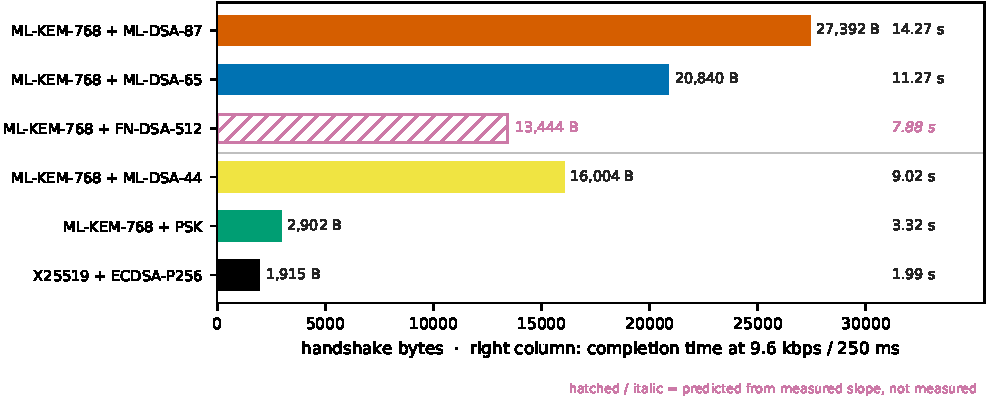
\includegraphics[width=\textwidth]{m4_ladder}
\caption{The byte-cost ladder. The hatched bar is the \fndsa{}-512
prediction; every other bar is measured, and the figure's own annotation
repeats the distinction. \fndsa{} is the smallest signature scheme
available and it does buy something --- 7.88\,s against 9.02\,s for
\mldsa{}-44, or 7.83--8.03\,s across the range of measured marginals ---
but the gain is 12.6\,\%, and it is smaller than the gain from dropping
one parameter set. Removing the certificate, at the bottom of the
figure, is worth 5.7\,s.}
\label{fig:ladder}
\end{figure}

The prediction is worth stating plainly because it contradicts the
intuition that smaller signatures are better. \fndsa{}-512 does buy
something: 7.88\,s against 9.02\,s for the already standardised
\mldsa{}-44, a gain of 12.6\,\%. But the gain is less than one step on
the \mldsa{} parameter ladder, and it is bought with three costs that do
not appear in the byte count. \fndsa{} signing on Cortex-M4 takes
19.6 million cycles in Pornin's constant-time implementation, about
117\,ms at 168\,MHz, against roughly 50\,ms for \mldsa{}-65
\cite{pornin2019falcon} --- a factor of 2.3 in the direction of the
computation we argued at the outset is not the bottleneck, but which
becomes relevant if the design is otherwise optimised. The expanded
private key needs 40--57\,kB of RAM, which is a substantial fraction of
the 192--512\,kB available on a typical flight controller. And
FIPS~206 has not been finalised, so a design that depends on \fndsa{}
depends on a moving target.

For completeness: \slhdsa{} is not a candidate here. Its smallest
parameter set carries 7{,}856-byte signatures (Table~\ref{tab:sizes},
from FIPS~205), 3.2 times the \mldsa{}-44 signature, and its signing
time is measured in hundreds of milliseconds on a microcontroller
\cite{pqm4}, against well under a millisecond for the lattice schemes.
Both costs are worse at every parameter set, and it is the right choice
only where hash-based assumptions are required, which is not the case
for a session handshake.

\subsection{Repeatability}
\label{sec:repeat}

The sweep in Table~\ref{tab:sweep} reports single runs, because a
9.6\,\kbps{} handshake takes long enough that repeating the full matrix
is expensive. To establish that the numbers are not noise, we repeated
the three configurations that carry the argument five times each
(Table~\ref{tab:repeat}).

\begin{table}[H]
\caption{Repeatability, five runs per configuration at 9.6\,\kbps{}
per direction and 250\,ms one-way, one batch. Byte counts are identical
across runs; time varies by less than 1\,\%. The individual runs are
kept in \texttt{results/repeatability\_raw.csv}, and two further batches
of the same kind are discussed below.}
\label{tab:repeat}
\centering
\begin{tabular}{lrrcr}
\toprule
Configuration & Bytes & Mean time (s) & SD (s) & Range (s) \\
\midrule
X25519 $+$ ECDSA-P256        & 1{,}916  & 1.989 & 0.013 & 1.967--2.002 \\
\mlkem{}-768 $+$ \mldsa{}-65 & 20{,}840 & 11.276 & 0.011 & 11.262--11.290 \\
\mlkem{}-768 pre-shared key  & 2{,}902  & 3.314 & 0.014 & 3.298--3.327 \\
\bottomrule
\end{tabular}
\end{table}

The standard deviations are 0.65\,\%, 0.10\,\% and 0.42\,\% of the
means, and the three means agree with the corresponding single runs in
Table~\ref{tab:sweep} to within 0.02\,s. The differences the paper
relies on --- 11.28 against 3.31\,s, or 9.02 against 11.27\,s --- are
two to three orders of magnitude larger than the run-to-run variation,
so the conclusions do not depend on measurement precision. The
1{,}916-byte classical figure here is one of the four baseline values
catalogued in Section~\ref{sec:attribution}; the byte-level
differences among them are DER encoding noise, not measurement error.

Two further batches of the same three configurations were run after the
table was compiled --- fifteen runs per configuration in total
(\texttt{results/repeatability\_raw*.csv}) --- and they say something
the single batch could not. \emph{The means reproduce; the spreads do
not.} Pooled over fifteen runs the means are 2.004, 11.285 and
3.340\,s, within 1\,\% of the table, but the coefficients of variation
rise to 4.6, 0.16 and 3.4\,\% because two of the forty-five runs
stalled: one pre-shared-key run at 3.74\,s against a 3.31\,s median, and
one classical run at 2.33\,s against 1.96\,s. Both are stalls of 0.4--0.5\,s
with no injected loss, which is the same order as the 0.446\,s that a
single retransmission costs in Section~\ref{sec:loss}. A batch of five
can miss such an event entirely, and the batch in
Table~\ref{tab:repeat} did; what protects the paper's conclusions is
that the smallest effect it resolves, the 20\,\% between \mldsa{}-65 and
\mldsa{}-44, is still four times the largest pooled coefficient rather
than thirty times the cleanest one. That is a narrower margin than the
first draft of this section claimed, and it is the honest one.

\section{Discussion}
\label{sec:discussion}

\subsection{Design Rules}

The measurements reduce to five rules, in descending order of value.

\textbf{Pre-provision trust if the operational model permits it, and
only if you already distribute symmetric keys.} This is worth
7.2$\times$ in bytes and 3.4$\times$ in time, and it is the only
intervention that brings a post-quantum C2 handshake within
1.67$\times$ of its classical cost. It is also the only one that
requires an architectural decision rather than a configuration change,
and the precondition is not decorative: the saving is airtime, while the
cost is a key-distribution mechanism the operator must already own.
Section~\ref{sec:alternatives} states when the option is unavailable and
Section~\ref{sec:keymgmt} when it is available but not worth buying.

\textbf{Do not spend effort on the key exchange.} The difference between
X25519 and \mlkem{}-768 is 2{,}200 bytes; the difference between
\mlkem{}-768 and \mlkem{}-1024 is a further 864. Both are small against
the 16{,}726-byte identity term, and \mlkem{}-768 is the right default
for a C2 link: category 3, and the ciphertext fits comfortably in the
objects the handshake already carries.

\textbf{Choose the certificate parameter set for security, not for
size.} \mldsa{}-44 saves 2.25\,s against \mldsa{}-65 at 9.6\,\kbps{}.
For scale, one retransmission on the same link costs 0.45\,s
(Section~\ref{sec:loss}), so the saving is worth about five losses:
real, but the kind of margin that a bad link day absorbs. If the
deployment requires category 5, \mldsa{}-87 costs 3.00\,s more than
\mldsa{}-65, also worth having measured, and a defensible price.

\textbf{Do not build on \fndsa{} for this application.} The 12.6\,\%
gain over \mldsa{}-44 does not justify a draft standard, a 2.3$\times$
slower signature, and 40--57\,kB of key state.

\textbf{Authenticate both directions, because it is free.} Removing the
client certificate halves the byte count --- 20{,}840 to 11{,}845 ---
and saves 0.10\,s of 11.28\,s, since the server's flight is the long
one and the client's certificate travels underneath it
(Section~\ref{sec:attribution}). Authenticating one direction only to
save airtime therefore buys 43\,\% of the bytes and 0.9\,\% of the
time. Spend the certificate at both ends.

\subsection{Why Not Simply Use Symmetric Keys}
\label{sec:alternatives}

The natural objection to the pre-shared-key recommendation is that it
assumes an operational model many UAV operators do not have. It is worth
being precise about where the recommendation applies, because the
boundary is what determines whether the paper is useful to a given
reader.

Pre-provisioned trust works when one organisation controls both
endpoints and can distribute key material out of band: a fleet operator
provisioning aircraft and ground stations, or a closed mission with a
fixed set of participants. In that regime the recommendation is not
merely available but obviously correct, and the classical baseline
already relies on it --- an operator running ECDSA today is relying on a
certificate infrastructure they control.

It does not work when the aircraft must establish a session with an
entity it was not provisioned against: a ground station operated by a
different organisation, an air traffic service provider, a UTM service,
or a relief aircraft from another fleet. Beyond-visual-line-of-sight
operations in controlled airspace require exactly this kind of
cross-organisational authentication, and there public-key cryptography
is not optional. For that case the certificate measurements of
Section~\ref{sec:sweep} apply, and the honest reading is that
certificate-based post-quantum C2 on a 9.6\,\kbps{} link costs about
eleven seconds per handshake. Whether that is acceptable depends on how
often the handshake happens, and session resumption is the obvious way
to keep it rare. It is worth measuring rather than assuming, and the
measurement corrects an earlier reading of our own: we had reported that
OpenSSL 3.5.7 cannot resume a \tls{}~1.3 session at all, because
\texttt{-sess\_in} re-ran the full handshake. That diagnosis was wrong in
its cause. \texttt{-sess\_out} works; what was missing was a ticket to
save. Every other measurement in this paper runs with
\texttt{-no\_ticket}, and a client that is never sent a
\texttt{NewSessionTicket} has nothing to resume.

With tickets enabled, resumption is measurable, but only for
server-authenticated handshakes. OpenSSL 3.5.7's \texttt{s\_server}
issues no ticket whenever client authentication is requested ---
\texttt{-verify 0}, \texttt{-Verify 0} and \texttt{-Verify 1} were each
tried, and a ticket appears only when client authentication is off
altogether. The reason is in the mode rather than in a bug: a resumed
\tls{}~1.3 handshake authenticates with the PSK and runs no certificate
authentication in either direction, so a server that requires a client
certificate on every connection has nowhere to get one from. RFC~8446
\cite{rfc8446} does not forbid the alternative --- a server may bind the
authenticated
client identity to the ticket and resume on that basis, and other stacks
do --- so this is a behaviour of one server implementation, and one more
reason to read the numbers here as stack-scoped
(Section~\ref{sec:threats}).

For the configuration in which it does work, measured on the same link:

\begin{itemize}
\item full server-authenticated handshake, 12{,}252 bytes and 11.26\,s,
      of which 352 bytes are the ticket itself;
\item resumed handshake, 3{,}335 bytes and 3.51\,s: 0.27 of the bytes
      and 0.31 of the time.
\end{itemize}

Three things follow, and the first two cut against resumption as a
substitute for the recommendation of Section~\ref{sec:psk}.

\textbf{Resumption is not cheaper than a bare pre-shared key.} The
external-PSK case of Table~\ref{tab:psk} costs 2{,}902 bytes and
3.31\,s; resumption costs 433 bytes and 0.20\,s \emph{more}, because
the ticket is carried on the first handshake and again on the resumed
one, while an operator holding a raw pre-shared key pays for neither.

\textbf{For mutual authentication, resumption is not available in this
stack at all.} An operator in the cross-organisational regime --- the
regime that needs certificates in the first place --- is running mutual
authentication, and on OpenSSL 3.5.7 that means no ticket and no
resumption. This is the paper's thesis showing up as a tool behaviour:
the moment trust is pre-provisioned, certificates stop going on the
wire, and a stack that must authenticate both directions by certificate
cannot get there by resuming.

\textbf{Where it does help, it helps a lot.} A 3.5\,s reconnect against
an 11.3\,s cold handshake is the difference between a session that can
be re-established per task and one that cannot. The usable deployment
is therefore server-authenticated transport with the aircraft's identity
carried at the application layer, where a ticket can replace the
handshake.

Three other alternatives are sometimes proposed and are worth
dispatching. Enlarging classical parameters is strictly worse: no
elliptic-curve parameter set resists Shor's algorithm. Quantum key
distribution does not fit the platform --- it needs a dedicated optical
channel, a fixed line of sight to a trusted node, and an authenticated
classical channel to bootstrap, which is the very problem it is supposed
to solve. And accepting the risk is a legitimate decision rather than an
oversight, provided it is made explicitly; Mosca's inequality
\cite{mosca2018} is the tool for making it explicit, and it requires an
estimate of migration cost, which is what this paper supplies.

\subsection{Chain Depth}
\label{sec:chain}

Every certificate in the tables above is self-signed, so the chain depth
is one. That is the right model for an operator who controls both
endpoints, and it is the model under which an operator would run
pre-provisioned trust anyway. It is not the model of a public key
infrastructure, where a leaf is typically accompanied by at least one
intermediate. We therefore built a two-level hierarchy --- root signing
an intermediate, intermediate signing the leaf, root trusted out of band
and never sent --- and measured it rather than extrapolating it.

The second link in the chain costs 11{,}248 bytes and 4.94\,s at
9.6\,\kbps{}: a two-level handshake measures 32{,}088 bytes and
16.22\,s against 20{,}840 and 11.28\,s at depth one
(Table~\ref{tab:chain}). The rule is linear in depth, since each
additional certificate is an independent list entry, so an operator with
\emph{n} intermediates should read every time in this paper as roughly
\mbox{11.28\,$+$\,4.9\,$\times$\,($n-1$)} seconds at this link rate.

\begin{table}[H]
\centering
\small
\caption{Depth one against depth two, same algorithm (\mldsa{}-65),
same link (9.6\,\kbps{}, 250\,ms), three repetitions each. Byte counts
are identical across repetitions because every certificate is generated
once and reused; the spread in time is 0.01\,s.}
\label{tab:chain}
\begin{tabular}{@{}lrrr@{}}
\toprule
Chain depth & Total bytes & Time (s) & vs depth one \\
\midrule
One (self-signed leaf)      & 20{,}840 & 11.28 & 1.00$\times$ \\
Two (leaf $+$ intermediate) & 32{,}088 & 16.22 & 1.44$\times$ \\
\midrule
Difference                  & $+$11{,}248 & $+$4.94 & \\
\bottomrule
\end{tabular}
\end{table}

\textbf{Where the 160 bytes beyond a naive estimate go.} A first
estimate treats the intermediate as a copy of the leaf and predicts
$2\times5{,}544=11{,}088$ bytes; the measurement is 11{,}248. The gap
resolves to the byte, and the resolution is worth recording because it
is a property of hierarchies rather than of this testbed. An
\mldsa{}-65 intermediate certificate encodes to 5{,}541 bytes, and each
\tls{} list entry adds a three-byte length and a two-byte extension
field, so the two intermediates account for 11{,}092. The remaining 156
bytes are the leaf growing from 5{,}514 to 5{,}592 bytes when it stops
being self-signed: a certificate that is verified against a parent
rather than against itself carries \texttt{extendedKeyUsage} and
\texttt{subjectAltName}, which the self-signed leaf does not need.
$2\times5{,}546+2\times78=11{,}248$.

\textbf{Why this is the more useful number.} The per-direction
figure can also be checked against the standard rather than against
another paper: an \mldsa{}-65 certificate carries a 1{,}952-byte public
key and a 3{,}309-byte signature \cite{fips204}, leaving 238 bytes for
names, validity and extensions, which is the 5{,}549-byte record of
Table~\ref{tab:records} once the three-byte \tls{} header is counted.
Both routes agree, which is what makes the depth-two result safe to
extrapolate further.

The direction of the error is the point. The absolute numbers in this
paper are what an operator with a flat, self-signed hierarchy would see.
An operator migrating a public hierarchy would see worse, and the
degradation is linear in chain depth --- which is a further argument for
flattening the hierarchy during migration rather than afterwards. Note
also that the 1.44$\times$ penalty for one extra link is larger than the
1.25$\times$ that the best signature-algorithm change buys
(Section~\ref{sec:sweep}): adding a certificate to the chain costs more
than every choice made inside it.

\subsection{The Operational Cost of Pre-Provisioning}
\label{sec:keymgmt}

The recommendation to pre-provision is easy to state and harder to
operate, and the difficulty is not cryptographic. Four problems
dominate.

\textbf{Provisioning.} Key material has to reach the aircraft before the
mission, through a channel that is itself trustworthy. Factory
injection covers the aircraft but not the ground stations or the relief
aircraft; field provisioning needs a mechanism and an audit trail, and
the moment that mechanism exists it becomes an attack surface that did
not exist when certificates were issued by a CA.

\textbf{Rotation.} A pre-shared key that is never rotated gives an
adversary unlimited time against a single compromise. Rotation requires
either connectivity at a known time --- which a beyond-line-of-sight
aircraft may not have --- or a key hierarchy that supports derivation,
which reintroduces some of the complexity the pre-shared key was meant
to remove.

\textbf{Revocation.} A certificate can be revoked and the revocation
distributed. A pre-shared key cannot be un-shared. If an aircraft is
captured, its key is compromised until every peer it could talk to has
been re-keyed, and the operator has to know which peers those were. The
magnitude is worth stating, if only as an estimate: twenty aircraft
against three ground stations is sixty pairwise keys, and the exposure
lasts until each of them has been replaced, which for the aircraft means
physical or out-of-band contact --- a maintenance action of an hour each,
so a sixty-hour campaign, and a window measured in weeks at the sortie
rate used above rather than in hours. The certificate case is not free
either, since a revoked chain still has to reach every station's
revocation list, but it is a distribution problem rather than a fleet
visit, and distribution completes in seconds over the same link that
carries the handshake.

\textbf{Scale.} A pre-shared key is pairwise. A fleet of $n$ aircraft
and $m$ ground stations needs up to $nm$ keys, or a group key with the
attendant problems of group rekeying. Certificates need one key per
node plus a trust anchor.

\textbf{The break-even, as arithmetic.} A pre-shared key saves 7.97\,s of
link time per handshake against the depth-one certificate path, and
12.88\,s once one intermediate is included. A small fleet --- twenty
aircraft flying twice a day, one handshake per sortie --- completes
14{,}600 handshakes a year and therefore saves 32 hours of airtime, or
52 with an intermediate. Both are about one working week. The trade
therefore does not turn on airtime at all: it turns on whether the
operator already runs key distribution. An operator who signs
\mav{}~v2 frames has that machinery already, because frame signing needs
a shared secret at both ends (Section~\ref{sec:background}); for them
the marginal cost of extending it upward to the handshake is a
configuration change, and the week of airtime is free. An operator who
does not --- one aircraft flown a few times a month --- will never
recover the cost of building it, and certificates remain the right
answer at any handshake rate. The threshold is a prior decision rather
than a fleet size, which is why this is an architectural question.

None of these is an argument against pre-provisioning; they are the
reasons it is an architectural decision rather than a configuration
flag. They are also the reason the alternative --- certificates, at
16.2\,s per handshake on a narrowband link once an intermediate is
included, against 11.3\,s without one --- remains the right answer for
open fleets, where the operational cost of pairwise key management
exceeds the airtime cost of a certificate chain. What this paper adds is
that the trade is now quantified: an operator weighing the two is
choosing between 3.3 and 11.3 seconds of link time per handshake, or
16.2 with one intermediate, and between a key-distribution problem and a
bandwidth problem.

\subsection{Relationship to Web-PKI Solutions}

The web has the same byte problem and is solving it structurally, by
batching many certificates under one signature so that a handshake
carries an inclusion proof rather than a chain
\cite{mtc2026draft,lec2026pq}. It is worth noting why that solution does not
transfer. Merkle Tree Certificates assume a client that caches
landmarks out of band and a certificate authority that issues in bulk;
a UAV fleet has neither, and the aggregation is over certificates from
one CA rather than over the two endpoints of one session. The UAV
analogue of the structural fix is not a Merkle tree but the pre-shared
key: both remove the per-session signature, but the pre-shared key
removes the certificate as well, which is where 87.9\,\% of the bytes
are.

\subsection{Threats to Validity}
\label{sec:threats}

\textbf{The link is emulated, not real.} The proxy reproduces
serialisation and propagation delay faithfully --- validated to
$+0.3$\,\% on a known transfer --- but it does not reproduce radio
fading, handover, or the queueing behaviour of a real satellite modem.
The clean-link numbers are not lower bounds, and the correction is
measured rather than assumed: at a 20\,\% per-segment loss rate
(Section~\ref{sec:loss}) completion time rises by 1.34\,s for the
certificate case against 0.45\,s for the classical one. The penalty
therefore grows with handshake size in absolute terms but shrinks in
relative terms, $+11.9$\,\% against $+22.8$\,\%, which is the
opposite of what one would guess, and it does not reorder the
architectures. Burstiness is bounded rather than measured:
Section~\ref{sec:loss} nets off the two errors, showing that correlation
of burst length $L$ divides the mean penalty by $L$ while leaving the
ratio between configurations unchanged, and that it lengthens the worst
stall from one RTO to $L \times 1.22$\,s. So the means here are an upper
bound, the tails a lower one, and the ranking holds either way. The link's
two other axes are swept rather than assumed: rate over 2.4--38.4\,\kbps{}
(Section~\ref{sec:rate}) and one-way delay over 0--600\,ms
(Section~\ref{sec:delay}), so the single-operating-point objection does
not apply to the ratio. What the delay sweep cannot settle is the
absolute value of its slope, which is a property of how the emulator
charges delay (Section~\ref{sec:delay}); only the ratio between
configurations is read from it.

\textbf{The computation is measured on the host, not on a flight
controller.} The arithmetic of the handshake was timed on the machine
that runs the testbed (Section~\ref{sec:scope}), which gives a margin of
three orders of magnitude rather than a cycle count for a specific part.
A reader who needs the latter has the literature \cite{pqm4,botros2019}
and a reason to think it does not change the conclusion: the margin is
wider than the gap between any published Cortex-M4 measurement and a
desktop core. Where the paper does use embedded figures --- the
\fndsa{} signing cost in Section~\ref{sec:compact} --- they are
attributed to the literature and used to argue against a design, not to
support one.

Two different questions are easy to conflate here, and this paper
answers only the first. \emph{Is the arithmetic affordable on a
microcontroller?} The margin says yes by three orders of magnitude, and
the literature measures it directly. \emph{Can a complete \tls{} stack
run on the flight controller at all?} That is a question about RAM,
flash, an operating system abstraction layer and a maintained port, and
nothing in this paper bears on it --- the stack measured here needs a
desktop operating system and would not be the one an airframe flew. An
operator whose avionics cannot host a \tls{} stack has a different
problem from the one this paper quantifies, and the pre-shared-key
recommendation of Section~\ref{sec:psk} is easier to satisfy at the
frame layer than at the session layer precisely because of that.

\textbf{One stack, one version.} All measurements use OpenSSL~3.5.7.
Another stack may frame records differently, and the 316-byte identity
overhead in the pre-shared-key configuration and the 2{,}200-byte key
exchange increment could move by tens of bytes. The 16{,}726-byte
identity increment is determined by the standards and would not move
materially.

\textbf{Single-run sweep.} Not every cell was repeated. The certificate
sweep of Table~\ref{tab:sweep} carries five runs per row, with standard
deviations of 0.024, 0.018, 0.012 and 0.013\,s --- coefficients of
variation of 0.62, 0.20, 0.10 and 0.09\,\%, the classical row being the
least stable for the reason Section~\ref{sec:attribution} gives. The
rate sweep of Table~\ref{tab:rate} is two runs per cell and the matrix
of Table~\ref{tab:matrix} is single-run, so those cells carry no
interval of their own. Elsewhere the five-run spreads of
Table~\ref{tab:repeat} are 0.10\,\% for the certificate handshake,
0.41\,\% for the pre-shared-key one and 0.67\,\% for the classical
baseline, though the pooled fifteen-run spreads of
Section~\ref{sec:repeat} are larger --- up to 4.6\,\% --- because two
runs in forty-five stalled. The smallest effect any table here is asked
to resolve is the 1.25$\times$ between \mldsa{}-65 and \mldsa{}-44, a
20\,\% difference, which is four times the largest pooled coefficient
and thirty times the cleanest one. Single runs are adequate for the
comparisons made at that resolution, and not for finer claims.

\textbf{The chain depth is one in the main tables.} All certificates
there are self-signed, so those numbers describe a flat hierarchy. The
depth-two case is not extrapolated: it was built and measured, and costs
11{,}248 bytes and 4.94\,s more per handshake, a factor of 1.44
(Section~\ref{sec:chain}). Depths above two are a linear extension of
that measurement rather than an independent one, and a public PKI with
cross-signing or multiple intermediates would sit above our depth-two
row. The reader should map our figures onto their own hierarchy rather
than treating them as worst cases.

\textbf{The \fndsa{} figure is a prediction.} It is labelled as such in
Table~\ref{tab:ladder}, Figure~\ref{fig:ladder} and the text, and it
rests on a slope measured over a range of 11.3\,kB that brackets the
predicted point. If a reader distrusts the extrapolation, the argument
survives on the measured \mldsa{}-44 point alone: 9.02\,s is already
close enough to \fndsa{}'s predicted 7.88\,s that the conclusion ---
compact signatures are not the lever --- does not depend on the
prediction.

\section{Conclusions}

Post-quantum migration of UAV command-and-control links is usually
framed as an embedded-computing problem: can the flight controller
afford \mlkem{} and \mldsa{}. Measured on a real \tls{}~1.3 stack over a
9.6\,\kbps{} beyond-line-of-sight link, it is an identity problem. Of the
20{,}840 bytes a mutual-authentication \mlkem{}-768\,$+$\,\mldsa{}-65
handshake puts on the wire, 18{,}310 are certificate and signature
material and 2{,}530 are key exchange. The smaller term is 12.1\,\% of
the total and the larger 87.9\,\%; driving the key exchange to zero ---
which no algorithm can --- would leave the identity term untouched.

The available remedies differ in value by a factor of three and a half.
(Times in this section are the single-run values of
Tables~\ref{tab:sweep} and \ref{tab:psk}, which differ from the
five-run means of Table~\ref{tab:repeat} by at most 0.02\,s; no
difference quoted here is affected.) Shrinking the signature scheme
from \mldsa{}-65 to \mldsa{}-44 saves
2.25\,s; extrapolating to \fndsa{}-512 saves a further 1.15\,s and
carries a draft standard, a 2.3$\times$ slower signature and 40--57\,kB
of key state. Removing the certificate entirely, by replacing
certificate authentication with a \tls{}~1.3 external pre-shared key,
saves 7.97\,s and brings the post-quantum handshake to within
1.67$\times$ of its classical cost.

The chain-depth measurement sharpens the same point from the opposite
direction. Adding one intermediate certificate costs 11{,}248 bytes and
4.94\,s, which is 2.2 times what the \mldsa{}-65 to \mldsa{}-44 change
saves. An operator who shrinks the signature scheme and then adds an
intermediate has made the handshake 2.7\,s worse than it started. The
lever is which certificates go on the wire, and how many, never how
large they are.

Resumption does not escape this. Measured on the same link, a resumed
handshake costs 3{,}335 bytes and 3.51\,s against 12{,}252 and 11.26 for
the cold server-authenticated handshake --- a third, and a real saving
--- but it is 433 bytes and 0.20\,s \emph{more} than the external
pre-shared key, which carries no ticket at all. And in the
mutual-authentication configuration that a cross-organisational operator
must run, OpenSSL~3.5.7 issues no ticket, so the option is not on the
table: a stack that has to authenticate both directions by certificate
cannot get there by resuming.

The rate sweep adds a correction that an earlier reading of these
numbers would have missed. The 5.66$\times$ above is the value at
9.6\,\kbps{}; holding propagation delay fixed and moving the rate from
2.4 to 38.4\,\kbps{}, the certificate penalty runs from 8.64$\times$
to 3.07$\times$. Migration therefore costs most on exactly the links
that have the least bandwidth to spare, and the pre-shared-key remedy
is worth 4.0$\times$ in time at the slow end against 2.5$\times$ at
the fast end.

The delay sweep closes the symmetric objection. Holding the rate fixed
and moving the one-way delay from 0 to 600\,ms, completion time is
linear in delay for all three configurations, but the certificate
handshake pays twice the slope of the classical one --- 4.00 against
2.03\,s per second of delay --- so the absolute gap widens from 8.80 to
9.99\,s. The ratio moves the other way, from 7.00$\times$ to
4.72$\times$, because latency is an additive term that dilutes a
smaller denominator faster than a large one. The net effect is that the
geostationary 5.66$\times$ is the mildest value any single-hop link
will see: a low-Earth-orbit path should expect 6.71$\times$ and the
zero-latency control 7.00$\times$, and only a two-hop path buys the
ratio down. The headline is therefore conservative for every link an
operator is likely to buy, which is the direction an error in a
migration study should point.

The design implication is uncomfortable but clear. The intervention
that matters is not an algorithm choice that a standards body will make
for the operator; it is an architectural choice the operator must make
themselves, about whether their aircraft needs to establish sessions
with parties they were not provisioned against. Operators who can answer
no should pre-provision and be done. Operators who must answer yes
should budget eleven seconds per post-quantum handshake on a narrowband
satellite TLS link over TCP, and at least that over DTLS, design
their session lifetimes accordingly, and watch
the Merkle-tree line of work with interest, because it attacks the same
byte budget from a different direction.

Two questions remain open. First, the loss model is independent and
memoryless. Section~\ref{sec:loss} bounds what correlation would change
--- the mean penalty falls as $1/L$ for a burst length $L$, the ratio
between configurations does not move, and a fade of $L$ segments stalls
for $L \times 1.22$\,s against the 1.2\,s this model can produce ---
but a measured Gilbert--Elliott trace on a real radio is still the
honest way to replace that bound. Second, the pre-shared-key
recommendation
assumes a key distribution mechanism we did not analyse; for a fleet,
that mechanism --- provisioning, rotation and revocation across
aircraft, ground stations and mission participants --- may itself be
the hard part, and it is a problem in operations rather than in
cryptography.

\vspace{6pt}

\authorcontributions{Conceptualization, <<A>>; methodology, <<A>> and
<<B>>; software, <<B>>; validation, <<A>>; formal analysis, <<A>>;
investigation, <<A>> and <<B>>; data curation, <<B>>;
writing---original draft preparation, <<A>>; writing---review and
editing, <<A>> and <<C>>; visualization, <<B>>; supervision, <<C>>;
project administration, <<C>>. All authors have read and agreed to the
published version of the manuscript.}

\funding{<<This research received no external funding.>>}

\institutionalreview{Not applicable.}

\informedconsent{Not applicable.}

\dataavailability{The measurement harness, the emulated-link proxy and
the record-layer parser are available at
\url{https://github.com/huanghuayu12/pqc-uav-drones}. The raw
measurements underlying
Tables~\ref{tab:breakdown}--\ref{tab:repeat} are stored as CSV and JSON
alongside them, and every figure in this paper is generated from those
files by the included plotting script.}

\conflictsofinterest{The authors declare no conflicts of interest.}

\abbreviations{Abbreviations}{%
The following abbreviations are used in this manuscript:\\

\begin{tabular}{@{}ll}
C2      & Command and Control \\
KEM     & Key Encapsulation Mechanism \\
PQC     & Post-Quantum Cryptography \\
PSK     & Pre-Shared Key \\
UAV     & Unmanned Aerial Vehicle \\
\end{tabular}}

\reftitle{References}

\bibliography{references}

\end{document}
